\chapter{Introduction}

% < Server: Microsoft-IIS/6.0
% < X-Powered-By: ASP.NET
% < X-AspNet-Version: 1.1.4322
This dissertation was submitted for registration over an unencrypted connection, to a web server running software that has passed end-of-life of security support.
Together with the dissertation itself, single sign-on credentials, useful to access all digital university systems, were submitted for authentication purposes.
All of this data neatly packaged and transmitted over an insecure connection, to a vulnerable remote host.

If you are a security researcher, you probably feel slightly distraught after reading the previous paragraph.
However, while being an inherently insecure situation, this is the reality of many systems today -- the system at the university is just one instance of a widespread problem of lack of cyber security.
Organizations maintain complex systems, at the same time as administrative responsibilities may be unclear, systems may be forgotten, or there may just be a mindset of ``if it is not broken, why fix it?''.
% if it ain't broke don't fix it
% if it is not broken, why fix it?
At the same time, 
%In the information society of today, information technology is constantly evolving in an ever increasing speed.
growing amounts of information and expectations of easy access increase the risk of information manipulation and leakage if systems are left vulnerable.

As the demand for increased computational power and storage has grown, there has also been a shift in how computer resources are consumed.
Traditionally, data has been stored and used on-premise, or at least on dedicated hardware bought and managed by the owner.
However, the current trend is to instead rely on computer resources managed and owned by someone else, commonly called \emph{cloud computing}.
This ubiquitous access to computer resources relieves the user from managing their own hardware, and reduces upfront costs for buying their own hardware.
It also allows for flexible scaling of resources, allowing the consumer to increase or decrease the consumed resources depending on workload, only paying for the actual resources consumed.

% 2) Some problems

The storage and use of information on remote resources do require a discussion about cyber security.
While outsourcing the maintenance of systems to a remote entity \emph{may} reduce the risk of ending up with unmaintained systems -- though very much dependent on the type of service bought -- it also introduces whole new classes of questions related to information security.
Some issues such as data ownership, availability guarantees, performance, and the type of service provided, can be solved by using Service-Level Agreements as legally binding contracts.
Such legal measures can allow customer compensation if the terms are not met, thus providing an incentive for the service provider to fulfil their promises.
However, legal approaches do only provide some mitigation \emph{after} an incident has occurred.

Consider the example of a leak of information from a cloud provider.
While the customer can demand compensation for a breach of contract, it does not change the fact that the information is now leaked and potentially distributed and publicly available.
The point is that legal agreements, while important in their own right, only go so far, since they mainly deal with mitigation, not prevention.
For the customer, the ideal situation would have been preventing the leak from occurring in the first place.

Preventive measures instead focus on trying to prevent such incidents from occurring at all.
Such measures can take many forms, including risk assessments, security policies, as well as purely technical measures used in the implementation of systems.
While all preventive measures are important and relevant, the focus of this dissertation will be different technical preventive measures.
In particular, the following areas are considered in more detail, and they can be used as preventive measures in the following ways.
\begin{itemize}
	\item Cryptography can be used to protect data at rest and during transmission, preventing information leakage.
	\item Trusted computing can be used to verify the integrity of code running remotely, preventing malicious code from processing information.
	\item Proactive approaches to assess software vulnerabilities can reduce the attack surface of deployed software, preventing attacks.
\end{itemize}

This dissertation presents technical contributions to several areas of the preventive measures described above.

\section{Dissertation Outline}

After this brief introduction and motivation to the scope of this work, the rest of the dissertation is structured as follows.
The following chapter, \chapref{ch:kappa-background}, provides both technical background, together with the current state of research in topics used throughout this dissertation.

In more detail, Section~\ref{sec:kappa-trustedcomputing} starts by presenting an overview of Trusted computing in general, together with technical background about several trusted computing technologies, as well as their potential applications.
This is followed by Section~\ref{sec:kappa-recommendersystems}, covering an overview of recommender systems, their possible applications in cyber security, and potential privacy implications of their use.
Third, in Section~\ref{sec:kappa-cryptography} we discuss the area of cryptography, with an emphasis on symmetric cryptography, stream ciphers in particular, and the analysis of such ciphers.

These three sections together present the background and context of the research contributions.
The contributions of each paper to the research field are described in Section~\ref{sec:kappa-contributions}, which is followed by some final conclusions and remarks in Section~\ref{sec:kappa-conclusions}.
Finally, in the second part of this dissertation, the individual included publications are presented in their published form, although reformatted for stylistic consistency with the rest of the dissertation.

\chapter{Background}
\label{ch:kappa-background}

This chapter presents some background from the various research fields of the contributions of this dissertation.
We start by presenting the area of trusted computing, which is then followed by recommender systems, and finally cryptography.

\section{Trusted Computing}
\label{sec:kappa-trustedcomputing}

In modern society, computers are ubiquitous and take part in our lives in many different ways.
While some of them are used directly by end-users -- devices such as desktop computers, laptops, or smartphones -- others are only used indirectly.
Such indirect use includes connecting to remote servers serving web pages, relying on your bank to maintain your account balances, and relying on your mobile phone network to service your calls.

Trusted computing is a technology to achieve \emph{trust} in a computer system.
The definition of trust here is important, and the Trusted Computing Group (TCG) defines it as follows:
\begin{quote}
```trust'  is  meant  to  convey  an  expectation  of  behavior'' \cite{TPM2.0r38}.
\end{quote}  
From this definition, we can restate the goal of trusted computing as guaranteeing a predictable behaviour of a computer system.
This is the definition that will be used throughout this dissertation when discussing trusted computing.

Providing such guarantees is important for the overall functionality of a system.
If the behaviour of crucial parts of the system is non-predictable, the behaviour of the system as a whole may be unknown.
Non-predictable behaviour may affect the security of the system as well; a subsystem performing unintended tasks may affect the confidentiality, integrity, or availability of data.

Trusted computing can be used both to guarantee the behaviour of local devices, but also to get guarantees of the behaviour of a remote system, thus covering all of the different types of devices mentioned in the beginning of this section.
Practical uses of protecting the system integrity of local devices include ensuring that a computer's software has not been modified since last use, and verification of the behaviour of remote devices, which can be especially relevant in a cloud computing context where the hardware is not controlled by the user.

A central concept in trusted computing is the reliance on a Trusted Computing Base (TCB), a set of hardware, firmware, and software critical to enforcing the security properties of a system.
Since the TCB is crucial to the guarantees provided by trusted computing, it is important that it behaves in the expected ways.
While this will be assumed for the remainder of this dissertation, we refer to techniques such as formal verification \cite{dsilva:2008,klein:2009,kern:1999} to actually achieve this important property.

\subsection{Attacker Model}
\label{sec:kappa-attackermodel}

For the work on trusted computing in this dissertation, the following attacker model is used.
The model is similar to attacker models of other works in trusted computing such as \cite{maene:2018,peters:2017}.
As described above in the definition of the TCB, trusted computing requires trust rooted in the hardware.
While software at any level (except software in the TCB) may be compromised by an attacker, the hardware is considered trusted and tamper-resistant from attackers throughout this dissertation.
In particular, the operating system may be compromised by an attacker, which means that access control policies provided by the OS may not be enforced.
An attacker may also eavesdrop on or modify traffic between systems, i.e. both passive and active network attacks can be performed.
Finally, we assume that cryptographic primitives such as symmetric and asymmetric ciphers, hash functions, and digital signatures are secure.

While all technologies requires some level of trust rooted in hardware, the extent of \emph{which} hardware components to trust differ between various trusted computing technologies.
Such details are discussed in connection to the description of each technology.

\subsection{Security Properties}
\label{sec:kappa-secprop}

When discussing trusted computing, it is helpful to look at smaller features, which will be used throughout the dissertation.
These features are called \emph{security properties}.
The following security properties will be used according to the definitions below, following definitions from earlier work such as \cite{maene:2018,vasudevan:2012}.

\begin{description}
	\item[Isolation]
	Also called isolated execution, ensures confidentiality and integrity of code and data inside an environment.
	Such an isolated environment is typically provided by hardware in a trusted computing setting.
	This feature ensures that someone outside the isolated environment cannot read or modify information inside the isolated execution environment.
	\item[Attestation]
	A property which allows a local or remote party to request proof that an application is in a certain state.
	This allows the verifying party to be confident in the integrity of an application.
	By extension, such integrity guarantees provides some guarantees of the behaviour of the attested code.
	While it does not guarantee that the code runs according to a written specification, it does provide a guarantee that it is indeed the expected binary implementation.
	\item[Sealing]
	A process of protecting the confidentiality of data such that it can only be read given that certain conditions are met.
	Common examples are sealing data to a particular hardware device, or to a certain state (cf. attestation above).
\end{description}

\subsection{Roots of Trust}

As described in the attacker model in Section~\ref{sec:kappa-attackermodel}, trust is generally rooted in some hardware component, either directly or indirectly.
A Root of Trust (RoT) can be different depending on the functionality it provides.
Among others, the TCG defines the following roots of trust, which have been chosen due to their relevance for this dissertation:
\begin{description}
	\item[Root of Trust for Measurement] The root from which measurement starts.
		There are two main ways to construct the base for measurements: either a Static Root of Trust for Measurement (SRTM), or a Dynamic Root of Trust for Measurement (DRTM).
		An example of SRTM is when measurement always starts at system startup.
		The measurements then include major parts of the system: BIOS, boot loader, kernel, etc.
		With DRTM, measurements can start at different points in time, but still give assurance that the system is in a known state.
	\item[Root of Trust for Reporting] Provides a RoT for attesting the origin and authenticity of a platform state, such as measurements.
	This is used during attestation of a system state.
	\item[Root of Trust for Storage] Provides a RoT for storage that protects both the integrity and confidentiality of data.
\end{description}

\subsection{Technologies}

To achieve the guarantees of trusted computing, there have been several different technologies proposed.
Each technology provides some set of the security properties described in Section~\ref{sec:kappa-secprop}, which are used to provide the guarantees of trusted computing.

The differences in selection of security properties provide us with several different technologies.
While all of them can be said to support trusted computing, they do so in different ways, are suitable for different use cases, and work on different hardware.
While this dissertation focuses on a few selected technologies, it starts with a brief overview of several currently existing technologies.
Later in this chapter some of them are described in more detail -- enough to provide a solid foundation for the discussion of the contributions in the dissertation.

The first technology to be discussed is the Trusted Platform Module (TPM).
The TPM is typically a discrete chip mounted on a motherboard, which together with software support can provide certain security properties.
A TPM can be used for attestation and sealing, but does not in itself provide an isolated execution environment.
Section~\ref{sec:kappa-tpm} covers TPM in more detail.

Looking at the class of commodity desktop, laptop, and server hardware using the x86 architecture, two well-known trusted computing technologies are Trusted Execution Technology (TXT) and Software Guard Extensions (SGX), both developed by Intel.
Intel TXT is described briefly in Section~\ref{sec:kappa-othertc}, but will not be covered in detail, instead we focus more on Intel SGX.

Intel SGX is a more recent development, only available on Intel x86 hardware.
In short, SGX allows isolated execution of code inside something called \emph{enclaves}.
The enclaves can be both locally and remotely attested, and both code and data can be included in measurements.
If desired, data can also be sealed.
SGX is discussed in more detail in Section~\ref{sec:kappa-sgx}.

While this dissertation will focus on the aforementioned technologies, some work in this dissertation is not necessarily limited to a specific technology for trusted computing, which makes it relevant to also briefly discuss alternative technologies.
A few other relevant technologies are mentioned later, in Section~\ref{sec:kappa-othertc}.

\subsection{Trusted Platform Module}
\label{sec:kappa-tpm}

The Trusted Platform Module (TPM) is a computer component, typically present as a discrete hardware component on the motherboard, which can perform various cryptographic operations.
This includes functionality such as encryption, signing, sealing, and attestation.
The functionality of a TPM is defined by the Trusted Computing Group (TCG) in their specifications, e.g., \cite{TPM1.2spec,TPM2.0r38}.
There are two main different versions of the specification in use today, TPM 1.2 and TPM 2.0, which differ in some areas.
However, both versions support the same general functionality.
Here we describe both versions, starting with TPM 1.2.

\subsubsection{TPM 1.2}
\label{sec:kappa-tpm12}

The first TPM 1.2 specification was released in 2003, with the most current revision of the specification being \cite{TPM1.2spec} released in 2011.
The TPM can be used to build a key hierarchy of asymmetric keys -- useful for signing or encryption -- where the root key of this hierarchy is called the Storage Root Key (SRK) and is stored inside the TPM.
The SRK can have child keys of different types, but all child keys are part of the key hierarchy by having their private key material encrypted by their parent's public key.
%Keys can either be generated internally inside the TPM, which ensures that the private key is only available inside the TPM, or the keys can be externally generated and then imported into the TPM.

Another important key of the TPM is the Endorsement Key (EK).
This key is a 2048-bit RSA key and is only generated once, usually before an end-user receives the module \cite{TPM1.2spec}.
The purpose of the EK is to have a Root of Trust for Reporting (RTR), so that an individual TPM can be authenticated.
This raises privacy concerns, since it means that an individual platform can be identified across services if the EK were to be used as the sole key.
To try to mitigate this issue, the TPM supports the use of Attestation Identity Keys (AIKs).
The purpose of the AIK is to allow the use of different keys for different context, to avoid the privacy issues of using a single key which uniquely identifies a TPM.

\paragraph{Platform configuration registers}

A TPM has at least 16 registers called Platform Configuration Registers (PCRs).
Each register can store a 160-bit hash value, suitable for holding the output of a SHA-1 hash.
The value of the PCRs are cumulative, such that after a reset (platform boot, or later), the updated value of a PCR with index $i$ is calculated as
\begin{align}
	\text{PCR}_i^{\text{new}} = h(\text{PCR}_i || \text{value})     \label{eq:kappa-pcrextend}
\end{align}
where $h$ is the hash function (SHA-1), and $\text{value}$ is the value to add to the PCR.

\paragraph{Attestation}

In TPM 1.2, attestation is performed by using an AIK together with PCRs.
Attestation of the platform is performed as follows.
During platform boot, the platform state is measured, for example firmware, bootloader, operating system, and configuration.
Measurements are cumulatively stored in the PCRs, which guarantees that if any part of the chain is modified, the resulting hash value stored in the PCR will be different.

To perform attestation, the PCR hash values -- which now represents the state of the platform -- are signed using the AIK.
This resulting package is called a \emph{quote}.
Since the AIK itself is tied to the very specific TPM it is loaded into, the quote can be verified by a local or remote entity, by first verifying the signature, and then inspecting the PCR values, which tells that the platform was in a certain state upon creation of the quote.

\paragraph{Migration}

While the TPM is designed to provide secure storage of keys, such that the private key material is protected by the TPM, it may be desirable to have the same key material on several different TPMs in certain circumstances.
An example of such a situation is when older hardware -- including the TPM -- is replaced, but encrypted data is to be retained.
This requires the new TPM to have the decryption keys from the older TPM.
Another situation is when designing a high-availability system with redundancy; each node then needs their own TPM with the required keys.

TPM 1.1 introduced \emph{migratable} keys to make it possible to migrate -- or rather duplicate -- keys to another TPM \cite{TPM1.1bspec}.
Keys can be marked as \emph{non-migratable} or \emph{migratable}, so that migration can be either disallowed or allowed.
To authorize the migration of a key, the TPM owner must authorize the destination, and the \emph{migration secret} must be presented to the TPM.
The implementation of non-migratable keys also uses this scheme; for a non-migratable key the migration secret is simply a secret value only known by the TPM (called tpmProof) thus making migration impossible to authorize for users.

TPM 1.2 further introduced another type of migratable key, called Certifiable Migration Key (CMK), which allows a third party to be in control over the destination of the migration.
This third party, the Migration Selection Authority (MSA), can be used to ensure that the destination of the migration is the intended, for example by checking that it is another TPM.

Migration, and scenarios where it is suitable, are also discussed in more depth when we make use of migratable keys as part of a solution to the problems discussed in \paperref{ch:tpmhas}.
We also discuss migration in \paperref{ch:tpm12to20} when we design a solution to migrate keys from TPM 1.2 to TPM 2.0.

\subsubsection{TPM 2.0}
\label{sec:kappa-tpm20}

TPM 2.0 is a newer version of the TPM specification \cite{TPM2.0r38}, and in many ways, TPM 2.0 is a generalization of TPM 1.2.
The key hierarchy has been replaced with a more general object hierarchy,
the use of RSA has been extended with support for several different types of cryptographic primitives,
and secrets have been partially generalized by the use of \emph{policies}.

As the changes between the old and the new standard are significant, there is no backwards compatibility with TPM 1.2.
The lack of such may require significant effort by system designers if a move from older TPM 1.2 hardware to newer TPM 2.0 hardware is desired.
Keys may require conversion, and the mismatch of features between TPM 1.2 and TPM 2.0 can cause issues with authorization, migration, and other tasks.
\paperref{ch:tpm12to20} of this dissertation tries to solve such issues by describing ways to achieve the old TPM 1.2 behaviour using the new functionality of TPM 2.0.

The goal of this section is to highlight some differences between TPM 1.2 and TPM 2.0 which will be important for the remainder of this dissertation.
For more details, refer to the specification \cite{TPM2.0r38}, or comprehensive guides such as \cite{arthur:2015}.

\paragraph{Duplication}

Migration has been renamed to \emph{duplication} in TPM 2.0, which is a more truthful description of the functionality, since the keys are indeed duplicated rather than moved.
There are also differences regarding the possibility to perform duplication in the first place.
While TPM 1.2 has migratable and non-migratable keys, TPM 2.0 has two new properties: \emph{fixedTPM} and \emph{fixedParent}, which is set on keys upon their creation.
If the former is set on a key, it is never allowed to leave the TPM.
If the latter is set, the key is fixed to its parent, and cannot be duplicated on its own, but might be duplicated indirectly if duplication of the parent key is allowed.

There is no longer a migration secret connected to keys in TPM 2.0, instead authorization is performed using the more general framework of policies, which will be described next.

\paragraph{Policies}

Policies is a new general authorization mechanism in TPM 2.0, which can be used to authorize several different operations on objects in the TPM.
As mentioned earlier, a policy can be used to authorize migration, but also to authorize for example regular usage of a key.
Policies work by including a value \texttt{authPolicy} into a key upon creation time.
The policy is calculated by building a hash chain of individual policy commands, called \emph{policy assertions}.
For an example see Figure~\ref{fig:kappa-tpm2policy} which outlines the idea.
\begin{figure}[ht]
	\centering
	\begin{tikzpicture}[scale=.75, every node/.style={scale=.75}, node distance=3cm, font=\sffamily]
		\node[]                           (zerostart)   {\texttt{000..00}};
		\node[draw,right=.75cm of zerostart]    (policypcr)   {\texttt{TPM2\_PolicyPCR}};
		\node[right=.75cm of policypcr]         (authpol1)    {\texttt{a53..1d}};
		\node[draw,right=.75cm of authpol1] (policyauth)  {\texttt{TPM2\_PolicyAuthValue}};
		\node[right=.75cm of policyauth]        (authpol2)    {\texttt{7c9..3a}};
		
		\node[above=.5cm of policypcr]     (pcrs)        {$\text{PCR}_i$};
		\node[above=.5cm of policyauth]    (authval)     {Auth value};
		
		\draw[->] (zerostart) -- (policypcr);
		\draw[->] (policypcr) -- (authpol1);
		\draw[->] (authpol1) -- (policyauth);
		\draw[->] (policyauth) -- (authpol2);
		
		\draw[->] (pcrs) -- (policypcr);
		\draw[->] (authval) -- (policyauth);
	\end{tikzpicture}
	\caption{Calculation of the \texttt{authPolicy} for a key requiring both PCR values and a secret value, called the auth value}
	\label{fig:kappa-tpm2policy}
\end{figure}
When calculating the policy hash, the TPM first starts with an all-zero hash, then for each consecutive policy assertion the previous hash value is concatenated with the output from the policy function, and then hashed again as:
\begin{align}
	\text{policyDigest}^{\text{new}} = h(\text{policyDigest } || \text{ policyAssertionOutput})
\end{align}
similar to how the PCR values are updated in (\ref{eq:kappa-pcrextend}).
The output from the policy assertion is based on the provided parameters.
Using \texttt{TPM2\_PolicyPCR} as an example, the output will depend on the selection and values of PCRs.
When the TPM performs access control, it executes the policy assertions, and then compares the calculated hash with the value stored in the \texttt{authPolicy} field of the object.

Since the \texttt{authPolicy} is a hash value, we note that the order of the policy assertions is important.
Evaluating two policy assertions in a different order will result in a different hash value.
Chaining several policy assertions in sequence means that both assertions need to be valid for the authorization to be true, thus it can be seen as a logical AND.
To realize a logical OR, a separate policy command is required, \texttt{TPM2\_PolicyOR}.
This policy assertion is true if any of the previous branches is true.

\begin{figure}[htbp]
	\centering
	\begin{tikzpicture}[node distance=0.3cm,auto,>=latex',scale=0.8, every node/.style={scale=0.8}]
	\matrix (m) [matrix of nodes, row sep=0.3cm]
	{
		\texttt{TPM2\_PolicyPCR}       &                  &  \\
		\texttt{TPM2\_PolicyAuthValue} &                  & \texttt{TPM2\_PolicySigned} \\
		&                  & \\
	};
	\path (m-2-1) -- (m-2-3) node[midway] (m-2-2) {}; % helper node for placing the node below.
	\node[below=0.5cm of m-2-2] (m-3-2) {\texttt{TPM2\_PolicyOR}};
	
	\draw[->] (m-1-1) to (m-2-1);
	\draw[->] (m-2-1) to (m-3-2);

	\draw[->] (m-2-3) to (m-3-2);
	\end{tikzpicture}
	\caption{Example of a policy chain with \texttt{TPM2\_PolicyOR}}
	\label{fig:kappa-tpm2policystructure}
\end{figure}

Throughout this dissertation, we will describe policy chains using figures similar to Figure~\ref{fig:kappa-tpm2policystructure}.
The final hash value, stored in the object's \texttt{authPolicy}, is the result of the evaluation of the final (bottom) policy, thus the figures should be evaluated from top to bottom.
Using Figure~\ref{fig:kappa-tpm2policystructure} as an example, access to the object is granted if \emph{any} of the following two conditions are met:
\begin{enumerate}
	\item The PCR values match some desired values \emph{and} a correct authorization secret is given.
	\item A valid signature can be provided over some parameter.
\end{enumerate}
By combining logical AND and logical OR in this way, it is possible to construct a wide variety of policy assertions.

\subsection{Intel SGX}
\label{sec:kappa-sgx}

\newcommand{\sgxcommand}[1]{\texttt{#1}}
\newcommand{\sgxadd}{\sgxcommand{EADD}}
\newcommand{\sgxcreate}{\sgxcommand{ECREATE}}
\newcommand{\sgxenter}{\sgxcommand{EENTER}}
\newcommand{\sgxexit}{\sgxcommand{EEXIT}}
\newcommand{\sgxextend}{\sgxcommand{EEXTEND}}
\newcommand{\sgxgetkey}{\sgxcommand{EGETKEY}}
\newcommand{\sgxinit}{\sgxcommand{EINIT}}
\newcommand{\sgxremove}{\sgxcommand{EREMOVE}}
\newcommand{\sgxreport}{\sgxcommand{EREPORT}}
\newcommand{\sgxresume}{\sgxcommand{ERESUME}}
\newcommand{\sgxmrenclave}{\sgxcommand{MRENCLAVE}}
\newcommand{\sgxmrsigner}{\sgxcommand{MRSIGNER}}

Intel Software Guard Extensions (SGX) is a set of instructions built into modern CPUs produced by Intel.
Being a trusted computing technology, it provides several different security properties, including isolation, attestation, and sealing.
By providing the different security properties within the processor itself, it is now enough to trust only the CPU vendor.
This is opposed to for example the TPM, which requires trust in both the TPM vendor for attestation purposes, and the processor that executes the machine code.

The instruction set was first proposed in 2013, separately describing isolated execution \cite{mckeen:2013}, and attestation and sealing \cite{anati:2013}.
The first hardware with support for SGX was shipped in 2015, starting with Intel's Skylake architecture.

Since SGX is an extension of the instructions supported by the CPU, applications can use SGX specific instructions to use the various security properties.
The most central concept in SGX is the \emph{enclave}.
An enclave is a trusted execution environment (TEE) where code and data can be loaded at creation time.
After creation, the code can be measured for attestation purposes, and execution of the enclave is done in isolation, so that no other process or enclave on the system can read its memory.

SGX2 is an extension to the original SGX specification, which adds a set of extra instructions related to SGX memory and thread management.
The instructions are described in great detail in \cite{intel64b}, but are not discussed here, since SGX2 has not been used in this dissertation.

The life cycle of an enclave is described next, followed by the security properties, and their specific implementation and usage in SGX.

\subsubsection{Enclave Life Cycle}

An overview of the life cycle of an enclave can be seen in Figure~\ref{fig:kappa-lifeofenclave}.
The enclave is first created using \sgxcreate{}, which creates internal structures with metadata about the enclave.
This is followed by repeatedly calling \sgxadd{} for each 4~KiB page of memory to add to the enclave.
This copies memory from unprotected memory into the EPC of the enclave.
If desired, \sgxextend{} can be called to measure 256 bytes of memory of the enclave.
The measurement will be stored in a measurement log, which can later be used to attest the integrity of the enclave.
\sgxextend{} needs to be repeated for every 256 byte block that should be measured.

When all desired pages has been added to the enclave, \sgxinit{} should be called to finalize the creation stage.
After this, no more pages can be added to the enclave, and the measurement of the added pages will be finalized.

After initialization, the enclave code can be executed.
This is done by calling \sgxenter{}, which starts execution of enclave code at a predefined location.
The enclave then continues execution until either a controlled exit occurs using \sgxexit{}, or until an exception or interrupt occurs, which will be handled by AEX.
To avoid clutter, the AEX flow is not described in Figure~\ref{fig:kappa-lifeofenclave}, but after AEX, execution can be resumed in the enclave by issuing \sgxresume{}.

\begin{figure}[t]
	\centering
	\begin{tikzpicture}[scale=1, every node/.style={scale=1}, node distance=3cm,
	ibox/.style={draw,minimum width=2cm},
	stagebox/.style={dashed,gray,opacity=0.5}]
	\node[ibox]                        (create) {\sgxcreate};
	\node[ibox,right of=create]        (add)    {\sgxadd};
	\node[ibox,right of=add]           (extend) {\sgxextend};
	\node[ibox,right of=extend]        (init)   {\sgxinit};
	\node[ibox,below=1.5cm of create]  (enter)  {\sgxenter};
	\node[ibox,right of=enter]         (exit)   {\sgxexit};
	\node[ibox,below=1.5cm of enter]   (remove) {\sgxremove};
	
	\coordinate (createadd)  at ($(create)!0.5!(add)$);
	\coordinate (addextend)  at ($(add)!0.5!(extend)$);
	\coordinate (extendinit) at ($(extend)!0.5!(init)$);
	\coordinate (initenter)  at ($(init)!0.5!(enter)$);
	\coordinate (exitremove) at ($(exit)!0.5!(remove)$);
	\coordinate (removedone) at ([xshift=0.25cm,yshift=0.25cm]remove.north east);
	\coordinate[above=0.25cm of extendinit |- extend.north east] (abovepos1);
	\coordinate (abovepos2)  at ([xshift=0.25cm,yshift=0.25cm]exit.north east);
	
	\coordinate (createentera) at ($(create)!0.4!(enter)$);
	\coordinate (createenterb) at ($(create)!0.6!(enter)$);
	\coordinate (enterremovea) at ($(enter)!0.4!(remove)$);
	\coordinate (enterremoveb) at ($(enter)!0.6!(remove)$);
	
	\draw[->] (create) -- (add);
	\draw[->] (add) -- (extend);
	\draw[->] (extend) -- (init);
	\draw[->] (init) |- (initenter) -| (enter);
	\draw[->] (enter) -- (exit);
	\draw[->] (exit) |- (exitremove) -| (remove);
	
	\draw[->] ([xshift=-0.075cm]extendinit) |- (abovepos1 -| extend) -| (addextend);
	\draw[->] ([xshift=+0.075cm]extendinit) |- ([yshift=0.15cm]abovepos1) -| (createadd);
	
	\draw[->] (exit.east) -| (abovepos2) -| ([xshift=-0.25cm]enter.north east);
	\draw[->] (remove.east) -| (removedone) -| ([xshift=-0.25cm]remove.north east);
	
	%\draw[dashed,gray] (createenter -| create.west) -- (createenter -| init.east);
	\draw[stagebox] ([xshift=-0.75cm]createentera -| create.west) rectangle ([xshift=0.25cm,yshift=0.75cm]init.north east);
	\draw[stagebox] ([xshift=-0.75cm]enterremovea -| enter.west) rectangle ([xshift=0.25cm]createenterb -| init.north east);
	\draw[stagebox] ([xshift=-0.75cm,yshift=-0.5cm]remove.south west -| remove.west) rectangle ([xshift=0.25cm]enterremoveb -| init.north east);
	
	\node[gray,left=0.75cm of create.west,anchor=north,rotate=90] {\footnotesize creation};
	\node[gray,left=0.75cm of enter.west,anchor=north,rotate=90] {\footnotesize use};
	\node[gray,left=0.75cm of remove.west,anchor=north,rotate=90] {\footnotesize teardown};
	
	\end{tikzpicture}
	\caption{Overview of enclave life cycle with instructions used in the creation, use, and teardown stage}
	\label{fig:kappa-lifeofenclave}
\end{figure}

\subsubsection{Isolation}

Recall that isolation, or isolated execution, means that code and data are stored within an isolated environment.
An entity outside the isolated environment should not be able to read or modify data within the environment.
This section briefly describes the various means SGX has to provide isolation.
For a more in depth description, refer to \cite{mckeen:2013} and \cite{intel64b}.

An interesting property of SGX is that enclaves provide isolation from other processes on the system, the operating system, hypervisors, as well as other enclaves.
This allows several -- potentially mutually distrusting -- enclaves to coexist on the same system while still providing isolation guarantees.

A special area of the system memory, called the Enclave Page Cache (EPC), is used by enclaves to store data.
This area cannot be accessed by peripherals, other enclaves, or other parts of the system, including hypervisors or operating systems.
This is enforced by the memory controller in the CPU, which uses the Enclave Page Cache Map (EPCM) structure which stores information about each page in the EPC.
The EPCM is then used by the processor to make access control decisions when enclave memory is accessed.
The contents of the memory is also encrypted so that enclave data is never stored in DRAM in plaintext, since the CPU is the only trusted agent in the SGX model.

To maintain isolation of the enclave, the entry and exit of enclaves is controlled and done with the \sgxenter{} and \sgxexit{} instructions, respectively.
This also ensures that the enclave can only be entered at predefined locations.
In case of an interrupt or an exception, the enclave will save its state securely using a process called Asynchronous Enclave Exit (AEX).
AEX ensures that an exception or interrupt handler in an untrusted domain outside the enclave cannot gain access to the internal enclave state.

\subsubsection{Attestation}

An important part of SGX is the possibility to perform attestation of enclaves.
A key component of attestation is to first get a measurement of the code and data of the enclave.
There are two important measurement registers related to attestation in SGX, \sgxmrenclave{} and \sgxmrsigner{}.
Both registers are 256 bit wide, and store SHA-256 hashes.
\sgxmrsigner{} is a hash of the public key that has signed the enclave, thus identifying the author, while \sgxmrenclave{} stores the hash of code and data that is included during enclave creation, which will be described more in depth below.

\sgxmrenclave{} is calculated during the creation of an enclave during the addition of pages to the EPC occurring between \sgxcreate{} and \sgxinit{}.
The measurement calculation is shown in Figure~\ref{fig:kappa-mrenclavecalculation}.
\begin{figure}[ht]
	\centering
	\begin{tikzpicture}[scale=0.8, every node/.style={scale=0.8}, node distance=3cm]
		\node[draw]                           (shainit)     {\texttt{SHA\_Init}};
		\node[draw,right of=shainit]          (shaupdate1)  {\texttt{SHA\_Update}};
		\node[     right=0.2cm of shaupdate1] (shaupdate2)  {\ldots};
		\node[draw,right=0.2cm of shaupdate2] (shaupdaten)  {\texttt{SHA\_Update}};
		\node[draw,right of=shaupdaten]       (shafinal)    {\texttt{SHA\_Final}};
		\node[draw,right of=shafinal]         (mrenclave)   {\sgxmrenclave{}};

		\draw[->] (shainit)    -- (shaupdate1);
		\draw[->] (shaupdate1) -- (shaupdate2);
		\draw[->] (shaupdate2) -- (shaupdaten);
		\draw[->] (shaupdaten) -- (shafinal);
		\draw[->] (shafinal)   -- (mrenclave);
		
		% dashed rectangles
		\node[draw,shape=rectangle,dashed,anchor=center,minimum width=2.7cm,minimum height=2cm] (shainitbox)    at (shainit.north)    {};
		\node[draw,shape=rectangle,dashed,anchor=center,minimum width=2.7cm,minimum height=2cm] (shaupdate1box) at (shaupdate1.north) {};
		\node[draw,shape=rectangle,dashed,anchor=center,minimum width=2.7cm,minimum height=2cm] (shaupdatenbox) at (shaupdaten.north) {};
		\node[draw,shape=rectangle,dashed,anchor=center,minimum width=2.7cm,minimum height=2cm] (shafinalbox)   at (shafinal.north)   {};
		
		\node[anchor=north] at (shainitbox.north)    {\sgxcreate{}};
		\node[anchor=north] at (shaupdate1box.north) {\sgxadd{}\texttt{/}\sgxextend{}};
		\node[anchor=north] at (shaupdatenbox.north) {\sgxadd{}\texttt{/}\sgxextend{}};
		\node[anchor=north] at (shafinalbox.north)   {\sgxinit{}};
	\end{tikzpicture}
	\caption{Overview of \sgxmrenclave{} derivation during enclave creation}
	\label{fig:kappa-mrenclavecalculation}
\end{figure}
The \sgxmrenclave{} measurement register is initialized during \sgxcreate{}.
Then, after each successive \sgxadd{} and \sgxextend{}, the hash is updated.
A call to \sgxadd{} will update the hash with metadata about the page that was added to the EPC, for example security properties, while a call to \sgxextend{} will update \sgxmrenclave{} with the content and metadata of a 256 byte data chunk.

SGX allows local attestation between enclaves on the same host, as well as remote attestation where an entity wishes to attest the integrity of an enclave running on a remote host.
This dissertation only considers the latter.
However, the local attestation sequence is relevant to understand how the remote attestation sequence works, thus both will be described below.

An overview of the local attestation flow can be found in Figure~\ref{fig:kappa-localsgxattestation}.
\begin{figure}[ht]
	\centering
	\begin{tikzpicture}[scale=1.0, every node/.style={scale=1.0}, node distance=3cm, font=\small\sffamily]
		\tikzset{circled/.style={draw,shape=circle,outer sep=2pt,inner sep=0.5pt,minimum size=0.35cm,font=\footnotesize,fill=white}}
		
		\node[draw,dashed,minimum width=9cm,minimum height=4cm] (userhost) {};
		
		\node[draw,solid,minimum width=3.2cm,minimum height=2.7cm,anchor=north west,below right=0.4cm and 0.4cm of userhost.north west] (appA) {};
		\node[draw,solid,minimum width=3.2cm,minimum height=2.7cm,anchor=north east,below left=0.4cm and 0.4cm of userhost.north east] (appB) {};
		
		\node[draw,solid,minimum width=2.4cm,minimum height=1.5cm,anchor=north,below=0.4cm of appA.north] (appAenclave) {};
		\node[draw,solid,minimum width=2.4cm,minimum height=1.5cm,anchor=north,below=0.4cm of appB.north] (appBenclave) {};
		
		\node[above=0.0cm of appA.south] {Application A};
		\node[above=0.0cm of appB.south] {Application B};
		
		\node[above=0.0cm of appAenclave.south] {Enclave A};
		\node[above=0.0cm of appBenclave.south] {Enclave B};
		
		\node[above=0.0cm of userhost.south] {Single host};
		
		\draw[<-] ([yshift=+0.5cm]appAenclave.east) -- node[above,circled] {1} ([yshift=+0.5cm]appBenclave.west);
		\draw[->] ([yshift=+0.0cm]appAenclave.east) -- node[      circled] {2} ([yshift=+0.0cm]appBenclave.west);
		\draw[<-] ([yshift=-0.5cm]appAenclave.east) -- node[below,circled] {3} ([yshift=-0.5cm]appBenclave.west);
	\end{tikzpicture}
	\caption{Overview of local attestation flow in SGX}
	\label{fig:kappa-localsgxattestation}
\end{figure}
The goal of the local attestation flow is for Enclave B to ensure that Enclave A is running on the same host as itself, that it is running inside an enclave, and that the expected code is running.
This is performed with the following steps \cite{anati:2013}:
\begin{enumerate}
	\item Enclave B sends its \sgxmrenclave{} value to Enclave A.
	\item Enclave A calls the \sgxreport{} instruction to generate a report structure, integrity protected using a MAC, containing data including \sgxmrenclave{} and \sgxmrsigner{}.
	The report is sent to Enclave B.
	Note that the key used to create this MAC is only known to Enclave B and the CPU itself, it is \emph{not} known by Enclave A.
	This proves that the report was created by trusted hardware, and not forged by Enclave A itself.
	\item Enclave B receives the report, and starts by verifying the MAC using its report key, retrieved by \sgxgetkey{}.
	If the MAC is valid, the contents of the report can be read, and Enclave B can verify the code and data integrity using \sgxmrenclave{} and \sgxmrsigner{}.
	If desired, Enclave B can now send its own report to Enclave A, if mutual attestation is desired.
\end{enumerate}

If we instead look at the remote attestation flow, a Verifier wishes to remotely attest an enclave running on a remote host.
An overview of the attestation sequence can be seen in Figure~\ref{fig:kappa-sgxattestation}.

\begin{figure}[ht]
	\centering
	\begin{tikzpicture}[scale=1.0, every node/.style={scale=1.0}, node distance=3cm, font=\small\sffamily]
		\tikzset{circled/.style={draw,shape=circle,outer sep=2pt,inner sep=0.5pt,minimum size=0.35cm,font=\footnotesize}}

		\node[draw]                                         (verifier)     {Verifier};
		\node[draw,right of=verifier]                       (application)  {Application};
		\node[draw,right of=application,align=center]       (enclave)      {Application\\Enclave};
		\node[draw,below=1.5cm of application,align=center] (qe)           {Quoting\\Enclave};
		\node[draw,below=1.5cm of verifier,align=center]    (ias)          {Attestation\\Service};
		
		\draw[->] ([yshift=+0.15cm]verifier.east) -- node[above,circled] {1} ([yshift=+0.15cm]application.west);
		\draw[<-] ([yshift=-0.15cm]verifier.east) -- node[below,circled] {6} ([yshift=-0.15cm]application.west);
		
		\draw[->] ([yshift=+0.15cm]application.east) -- node[above,circled] {2} ([yshift=+0.15cm]enclave.west);
		\draw[<-] ([yshift=-0.15cm]application.east) -- node[below,circled] {3} ([yshift=-0.15cm]enclave.west);
		
		\draw[->] ([xshift=+0.15cm]application.south) -- node[right,circled] {4} ([xshift=+0.15cm]qe.north);
		\draw[<-] ([xshift=-0.15cm]application.south) -- node[left,circled]  {5} ([xshift=-0.15cm]qe.north);
		
		\draw[<->] (verifier.south) -- node[right,circled] {7} (ias.north);
		
		% dashed rectangle and label.
		\draw[dashed] ([xshift=0.25cm,yshift=0.25cm]enclave.north east) rectangle ([xshift=-0.5cm,yshift=-0.25cm]qe.south west);
		\node[below=1.5cm of enclave] (remotehost) {{Remote host}};
	\end{tikzpicture}
	\caption{Overview of remote attestation flow in SGX}
	\label{fig:kappa-sgxattestation}
\end{figure}

%\noindent
The numbered steps in the figure corresponds to the following steps in the attestation flow \cite{anati:2013}:
\begin{enumerate}
	\item The Verifier issues a challenge to the remote host, challenging it to prove that it runs code inside an enclave.
	\item The (untrusted) application forwards the challenge, together with the identity of the Quoting Enclave to the Application Enclave.
	The Quoting Enclave is an Intel-provided enclave.
	\item The Application Enclave calls the \sgxreport{} instruction to generate a report structure, integrity protected using a MAC, containing data such as \sgxmrenclave{} and \sgxmrsigner{}.
	The report is generated by the CPU, using a key only accessible to the CPU and the Quoting Enclave.
	The report is sent back to the application.
	\item The report is forwarded to the Quoting Enclave.
	\item The Quoting Enclave verifies the report by checking the MAC using its report key, retrieved by \sgxgetkey{}.
	If the MAC is valid, it creates a quote structure, containing the report and then signs the quote with a private platform-specific private key, using the EPID scheme \cite{brickell:2010}.
	Since this is a group signature scheme, it allows the creation of signatures without revealing the identity of the signing CPU.
	\item The signed quote is sent back to the Verifier.
	\item The Verifier can now verify the EPID signature of the quote by contacting an attestation service, typically the Intel Attestation Service (IAS), to ensure that the signature of the quote is valid. If it is, it can extract the \sgxmrenclave{} and \sgxmrsigner{} fields and compare them to known good values.
\end{enumerate}
After these steps, the Verifier can be sure that the enclave is: running inside an enclave on genuine hardware, and that the code and data in the enclave has not been modified before it was started.
These guarantees hold as long as the Verifier accepts the trust model of SGX.
Note that the communication between Application Enclave and Quoting Enclave is the local attestation flow described earlier, where the Quoting Enclave wishes to attest the Application Enclave.
Only if this local attestation is valid, the Quoting Enclave will sign the quote and pass it on.

For a more in depth description of attestation refer to \cite{anati:2013} and \cite{intel64b}.

\subsubsection{Sealing}

While the enclave protects the integrity and confidentiality of data while the enclave is running in memory, it can also be desirable to persist data to non-volatile media before the enclave exits.
This can be done by using sealing, which can be performed using several different policies in SGX.

Regardless of policy, the \sgxgetkey{} instruction is called together with the desired policy, and a 128-bit key is derived and returned by the CPU.
The key can then be used for encryption and/or integrity protection of data, before the data is persisted to disk.
Also, regardless of policy, the derived keys are unique to the particular CPU that derives the key; two identical enclaves running on different CPUs will derive different keys.
The sealing policies can be categorized into two major categories depending on the measurement register the key derivation is based on: either \sgxmrenclave{}-based or \sgxmrsigner{}-based.

In the first case, the sealing key will only be available to enclaves with the same \sgxmrenclave{} hash.
This ensures that only a particular enclave implementation will be able to unseal the data.
However, this also means that an updated version of the enclave, for example with security patches, will not be able to unseal data from a previous enclave version.

In the second case, the sealing key will be based on the \sgxmrsigner{} hash, together with a product id, and security version number (SVN).
The SVN can be used to allow an upgraded enclave to access sealed data from a previous version of the enclave.
This makes the management of security patches easier, since sealed data is accessible to newer enclave versions.
It is also possible to seal data without a product id, thus making it possible to share data between different enclaves from the same vendor.
For more details about sealing policies, refer to \cite{anati:2013} and \cite{intel64b}.

\subsubsection{Attacks on SGX}

Since the design of SGX was made public, there has been a progression in research related to potential attacks.

Several attacks have considered side-channel attacks related to memory management in Intel SGX, starting with the discussion of lack of protection against side-channel attacks in \cite{costan:2016}.
Fairly soon after these realizations, side-channel attacks on SGX started to appear.
In \cite{gotzfried:2017} the authors show a practical attack that can extract the AES key used for decryption inside an SGX enclave.
The attack is based on cache-timing attack, and can extract the AES key in less than 10 seconds, and is performed outside the enclave, thus breaking the isolation property of SGX.

Other attacks include \cite{schwarz:2017}, which performs an attack on an RSA implementation running within an enclave.
The attack is performed from within an attacker enclave, and attacks another enclave running on the same host.
It manages to recover the private RSA key either partially with a single trace, or completely when using multiple traces.
Similarly, \cite{brasser:2017} shows that the recovery of a private RSA key is possible, as well as the recovery of potentially sensitive genome data.
The extent of potential side-channel attacks is also discussed systematically in \cite{wang:2017}.

One way to avoid side-channel attacks is to implement algorithms in a data-oblivious way.
In \cite{ohrimenko:2016} this is discussed in the context of machine learning algorithms running inside SGX, where the authors propose data-oblivious algorithms for several common machine learning methods.
Also on the defensive side, \cite{gruss:2017} presents \emph{Cloak}, a technique to prevent attackers to observe cache misses.
The overall idea is to use hardware transactional memory, such as Intel TSX, which can be used to ensure that certain memory stays in the processor cache for the duration of the calculations, thus preventing cache-timing attacks.
The performance overhead is however heavily dependent on the amount of memory accesses in the code.

However, the previously mentioned mitigation does not always work.
In \cite{vanbulck:2018} the authors present Foreshadow, an attack based on the ideas from the Meltdown attacks \cite{lipp:2018}, but applied to SGX.
The attack leaks information from within the enclave, and also attacks the architectural enclaves such as the Quoting Enclave.

While the envisioned use case for SGX is to run trusted code within an enclave, shielding it from the unprotected world outside of SGX, \citeauthor{schwarz:2019} show that malware can be executed within an enclave \cite{schwarz:2019}.
Because of the isolation property of enclaves, such malware enclaves may avoid detection from anti-malware software running on the host.

%\cite{brasser:2017} % builds on others, easy to deploy, avoid detection rsa decryption, genomic processing
%\cite{gotzfried:2017} % 
%\cite{schwarz:2017}
%\cite{wang:2017} % considers many different sc in a systematic approach.
%\cite{gruss:2017}
%\cite{vanbulck:2018} % immune to gruss:2017 (cloak)
%\cite{schwarz:2019}

\subsection{Other Trusted Computing Technologies}
\label{sec:kappa-othertc}

While the previous sections have discussed trusted computing technologies used later on in this dissertation, it is also valuable to briefly discuss other potential options.
The main motivation behind this is that some contributions are not necessarily tied to a specific trusted computing technology, but could be implemented by using several others as well, as long as they provide the required combination of security properties.

One technology is Intel TXT, which allows the use of a DRTM for an execution environment \cite{TXT-mle}.
It allows for an application or operating system to launch a Measured Launch Environment (MLE) of trusted code.
Intel TXT uses the PCR values of the TPM to store measurements, together with new instructions to actually perform the launch of the MLE.

Related to the TPM, one variant of the TPM is the Mobile Trusted Module, based on the TPM 1.2 specification, but with adoptions for mobile use cases.
The specification can be seen in \cite{MTM1.0spec}, and for an overview of the functionality the reader is referred to \cite{ekberg:2007}.
There has been several proposed options for actual MTM implementations, for example implementations based on TrustZone (described next) \cite{winter:2008}, M-Shield \cite{ekberg:2009}, or as a physical chip \cite{kim:2010}.

Another technology is ARM TrustZone, available in ARM processors starting with ARMv6 in 2002 \cite{zhang:2016}.
TrustZone provides two different worlds: a secure world, and a normal world.
The normal world runs a regular, rich, operating system as well as all other regular software installed on the system.
The secure world typically runs a specialized trusted software stack, implementing the desired security features.
The processor ensures that software in the normal world cannot access memory of the secure world, while the secure world has access to all memory: both in the secure and normal world.

Other trusted computing technologies focus on other platforms, such as Sanctum \cite{costan:2016b} for RISC-V, SecureBlue++ \cite{boivie:2013} for POWER, and Bastion \cite{champagne:2010} for OpenSPARC.
For surveys of other technologies, we refer to for example \cite{zhang:2016,peters:2017,maene:2018}.

The different trusted computing technologies each provide a different API, and different ways to use the security properties they provide.
Ongoing efforts to abstract differences between different technologies include for example Asylo \cite{asylo} and Open Enclave \cite{openenclave}.

\subsection{Research on Trusted Computing}

With the previous sections describing the background of the various trusted computing technologies, this section describes research trends as well as potential applications of the technology.
Research on trusted computing covers a wide area, and can have applications both on client-oriented devices, as well as in more server-oriented use cases.

On client-oriented devices, BitLocker \cite{Bitlocker} is perhaps the most well-known use of the TPM today, being available in certain Windows versions since the launch of Windows Vista in 2007.
BitLocker is a disk encryption solution, and can use TPM sealing such that the disk encryption keys are only released when the boot environment is unmodified.

On mobile devices, where use of ARM processors is widespread, use of TrustZone is most common.
Examples include the use of TrustZone in the Android Keystore \cite{androidkeystore}, and Samsung Knox allowing containers, useful to, e.g., separate business and personal containers on a single device \cite{kanonov:2016}.
TrustZone can also be used as a trust root to implement other technologies.
An example is the Mobile Trusted Module which can be implemented by the use of TrustZone as a root as in \cite{winter:2008}.
While interesting, we will not consider such client-oriented applications further in this dissertation, and instead focus on more server-oriented use cases.
We first related to virtualization and cloud computing, followed by privacy-preserving measures.

\subsubsection{Virtualization and Cloud Computing}

There has been a lot of focus on the use of trusted computing technologies in the area of virtualization and cloud computing.
Starting with the TPM, which in itself is not trivially shared between multiple virtualized machines, \citeauthor{berger:2006} proposed virtualization of TPMs, vTPM, in \cite{berger:2006}, allowing virtual TPMs to be connected to virtual machines at the same time as trust in the vTPMs is rooted in the single hardware physical TPM.
Other approaches include para-virtualized TPM sharing \cite{england:2008}, and property-based TPM virtualization \cite{sadeghi:2008}.

A possible benefit of the cloud infrastructure is the possibility to increase availability.
Migrating services between different physical hosts allows flexibility of hardware maintenance, and is an import part of a cloud service.
However, migration introduces difficulties when combined with TPMs (both physical and virtualized), because of the underlying change in physical host.
The problems are discussed in papers such as \cite{danev:2011} and \cite{wan:2012}.

In \paperref{ch:tpmhas} we also consider the availability problem by describing the use of TPMs in a high-availability system (HAS).
Instead of a virtualization approach, we instead consider a system with multiple, independent, computational units (CUs) which together constitute the HAS.
We propose a solution for how each TPM-equipped CU can share the same keys required to decrypt secure storage for availability purposes, by describing a key migration scheme using the functionality in either TPM 1.2 or TPM 2.0.

In \paperref{ch:tpm12to20} the key migration features of both TPM versions are discussed in depth, as we design a way to migrate key material from TPM 1.2 to TPM 2.0, thus allowing the migration from old to new hardware while keeping the same keys.
Due to the lack of backwards compatibility between the two versions, this requires careful considerations to maintain the same key material and behaviour with regard to authorization.

Since SGX was presented in 2013, it has attracted much attention in virtualization and cloud computing.
Proposed use cases include distributed MapReduce computations while maintaining confidentiality and integrity \cite{schuster:2015}, shielded execution of applications in the cloud \cite{baumann:2015}, running Docker containers inside enclaves \cite{arnautov:2016}, and secure database engines \cite{priebe:2018}.

Network function virtualization (NFV) and Software-Defined Networking (SDN) are two technologies often used together with virtualization and in the cloud, since they allow an increased flexibility with regard to network management.
For an overview of respective technology, the reader is referred to \cite{casado:2014} and \cite{mijumbi:2016}. % first is for SDN, second for NFV + connection to SDN.
While security in SDN networks is a broad topic in itself, there has been previous research discussing trusted computing technologies in connection with SDN.
Examples include the discussions of securing inter-domain routing in \cite{kim:2015}, securing NFV states in \cite{shih:2016}, and a framework to securely bootstrap virtual network infrastructure in SDN \cite{paladi:2016b}.
In \paperref{ch:trustanchors} we also present contributions to the security in SDN networks, by presenting work protecting credentials and cryptographic context of network elements, as well as a secure enrollment mechanism for network elements in a software-defined network.
For both parts, we utilize trusted computing technologies.

\subsubsection{Privacy-preserving Computations}

The isolation guarantees of SGX are also interesting from a privacy-preserving perspective.
Performing privacy-preserving computations can be performed in many ways, including fully homomorphic encryption \cite{gentry:2009}, secure multiparty computation \cite{yao:1982}, and lastly by using trusted execution environments, which will be the focus of this section.

Privacy-related topics where SGX have been used are, e.g., a framework for MapReduce computations \cite{schuster:2015}, a sandbox to perform arbitrary calculations on secret data \cite{hunt:2018}, functional encryption \cite{fisch:2017}, multiparty computations \cite{kucuk:2016,bahmani:2017}, private web search \cite{mokhtar:2017,pires:2018}, and in machine-learning settings \cite{ohrimenko:2016,chandra:2017,hunt:2018b}.

In \paperref{ch:recsyssgx} we also use Intel SGX to design a privacy-preserving system, but in the context of a recommender system (recommender systems in general, and privacy in recommender systems in particular will be discussed shortly, in Section~\ref{sec:kappa-recommendersystems} and \ref{sec:kappa-recsysprivacy}, respectively).
In this recommender system, sensitive information consist of the user profiles, which are protected by designing an intermediary, running inside an SGX enclave.
The design using an intermediary is similar to the work presented in \cite{lie:2017}, where the intermediary is verifiable by the client before it is entrusted with sensitive information.
In contrast to our work, the targeted recommender system is different, where \paperref{ch:recsyssgx} considers a recommender which is not collaborative, which makes the use of validation predicates unnecessary -- malicious input would only affect the profile of the user itself.
Instead of blinding by combining multiple inputs, we derive pseudo profiles, used to issue fake queries together with the genuine query, similar to the approach discussed for private web search in \cite{mokhtar:2017}.

\newpage
\section{Recommender Systems}
\label{sec:kappa-recommendersystems}

The general goal of a recommender system is to provide recommendations from a set of items to some user, the idea being that the recommendations are adapted to the user's interests or needs.
Recommender systems are widely used in a lot of different scenarios, including e-commerce, music, videos, social media, and many others.
The common denominator is that there is a large set of content, such as books, songs, videos, or social media posts -- more than the user can or wishes to manually browse.
The purpose of a recommender is to filter this large set, which likely contains many items not relevant for the user, and present the filtered view to the user to further interact with.

The end goal of presenting this filtered view can be one of many, a few examples are listed below:
\begin{itemize}
	\item In an e-commerce setting, the goal is to increase the sales.
	By providing recommendations that the users are likely to be interested in, or at least likely to buy, the revenue of the seller can increase.
	\item For a monthly fixed-rate streaming service for music or videos, the goal may be to increase user satisfaction by providing recommendations of new or old content.
	\item For content financed with advertisements, the goal of the recommender could be to increase the ad revenue by recommending interesting content to the users, increasing the chance that they stay on the service and are exposed to more advertisements.
\end{itemize}

A conceptual view of a recommender system can be seen in Figure~\ref{fig:kappa-recommender}.
The recommender takes two inputs: user information and item information.

\begin{description}
	\item[User information] This can be any kind of information about a user, and the information can be supplied both explicitly and implicitly by the user.
	Examples of explicit user information would be user-stated preferences or properties such as interests, ratings, or age.
	Implicit user information could instead be automatically collected data about users, such as visited web pages, or purchase history.
	\item[Item information] This is instead information about the set of possible items to recommend.
	This is highly dependent on the items in question, but common examples are price, manufacturer, and product type, in case of a recommender system for manufactured goods.
\end{description}

\begin{figure}[tb]
	\centering
	\begin{tikzpicture}[scale=1, every node/.style={scale=1}, node distance=1cm, font=\small\sffamily,
	database/.style={
		cylinder,
		shape border rotate=90,
		aspect=0.15,
		draw
	}],
		\node[draw,align=center]                             (recommender)     {Recommender\\system};
		\coordinate[left=2cm of recommender,anchor=east]     (midpoint);
		\node[database,above=0.5cm of midpoint,align=center] (userinfo)        {User\\information};
		\node[database,below=0.5cm of midpoint,align=center] (iteminfo)        {Item\\information};
		\node[right=of recommender]                          (recommendations) {Recommendations};
		
		\draw[->] (userinfo)    -- (recommender);
		\draw[->] (iteminfo)    -- (recommender);
		\draw[->] (recommender) -- (recommendations);
	\end{tikzpicture}
	\caption{Conceptual view of a recommender system}
	\label{fig:kappa-recommender}
\end{figure}

The recommender system combines user and item information, and outputs a set of recommendations, which is a subset or ranking of items that is likely to be relevant to the user in question.
The output can be of many forms, some common examples include:
\begin{itemize}
	\item A subset of all items, such that the subset contains items relevant to the user.
	\item A ranking of items, such that items are ordered according to their perceived relevance to the user.
\end{itemize}

Recommender systems can generally be categorized depending on the internal method used to generate the recommendations \cite{aggarwal:2016}.
Three major methods are: knowledge-based methods, content-based methods, and collaborative filtering methods.
They are described in more detail in the following sections.

\subsection{Knowledge-based Methods}

In a knowledge-based recommender system, the input of the recommender takes the form of user \emph{requirements} and item information, together with knowledge of the domain the recommender works in.
A distinctive feature of this type of recommender is that it does not work with user ratings or user history from previous interactions, but rather with a set of user-specified requirements.

There are two major classes of knowledge-based system, case-based and constraint based \cite{ricci:2011}. 
Case-based systems are based on a similarity function, which calculates the similarity between the desired item (user requirements), and items actually available.
Constructing the similarity function requires knowledge of the domain in question, but after construction it can be used to support several different interfaces.
The user can either specify individual requirements directly, or they can request items similar to other items.
Both interfaces are possible because they both use a similarity function.

The other class is constraint-based systems.
In these systems, the user typically provide their requirements in the form of constraints.
In case of a house or an apartment, it could be the minimum and maximum number of rooms, living area, etc.
The constraints do not have to explicitly map to item attributes; the designer of the recommender system can use domain-specific rules to map between user requirements and item attributes.
Compared to case-based systems above, the main difference lies in how case-based systems use a similarity function, while constraint-based systems use a set of rules that defines the mapping from requirements to items.

In general, knowledge-based systems are suitable in situations where items are bought rarely, such as cars, houses, apartments, and similar expensive items \cite{aggarwal:2016}.
In these cases, it can be hard to gather enough history of purchase to generate suitable recommendations.
Requirements may also change with time, consider the previous example of a recommender for real estate; it is very likely that the user's preferences have changed since the last time they bought a house or an apartment -- after all, there is a reason they are looking for something new.
Knowledge-based systems solve this by not trying to learn from past user behaviour, instead focusing on their current requirements, and use domain-specific knowledge to try to compare these requirements to item attributes.

\subsection{Content-based Methods}

Content-based methods take the individual history of the user into account when generating recommendations.
By considering the user's rating of previous items, the recommender tries to find similar items that the user may like.
This is done by comparing the attributes of previously liked items, and finding other items with similar attribute values.
A typical example is a movie recommender system, where a user has given a movie a high rank.
The recommender will then look at the attributes of the movie, and then try to find other movies with similar attributes, and presents these movies to the user.

Content-based systems have both advantages and disadvantages \cite{aggarwal:2016}.
Advantages include that newly added items can be recommended, since their attributes can be compared with older items immediately.
On the contrary, a well-known disadvantage is that new users cannot be given any reasonable recommendations, since they have not yet rated any item.
This is an example of the cold-start problem of recommender systems.

\subsection{Collaborative Filtering}

Collaborative filtering methods are typically designed around a rating matrix, such as the matrix in Figure~\ref{fig:kappa-cf}.
The rating matrix is sparse, and contains the ratings from a user $u_a$ of an item $i_b$.
Generating recommendations can now be seen as filling out this sparse matrix, such that unknown ratings are estimated by using data from other parts of the matrix.
An important distinction between collaborative filtering methods and previously described methods is that collaborative filtering also considers information from \emph{other} users of the system.

\begin{figure}[ht]
	\centering
	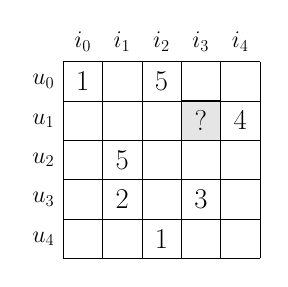
\begin{tikzpicture}[scale=0.5, every node/.style={scale=0.5}, node distance=1cm]
		\draw[step=1cm,very thin] (0, 0) grid (5, 5);
		
		\foreach \x in {0,...,4}
			\node at (\x+0.5, 5.5) {\LARGE $i_{\x}$};
		\foreach \y in {0,...,4}
			\node at (-0.5, 4-\y+0.5) {\LARGE $u_{\y}$};
		
		\draw[fill=gray!20] (3,3) rectangle (4,4);
		
		\foreach \x/\y/\v in {3/1/?, 1/2/5, 3/3/3, 0/0/1, 1/3/2, 4/1/4, 2/0/5, 2/4/1}
			\node[] at (\x+0.5, 4-\y+0.5) {\huge \v};
	\end{tikzpicture}
	\caption{Example of a rating matrix used in collaborative filtering}
	\label{fig:kappa-cf}
\end{figure}

Consider the rating matrix in Figure~\ref{fig:kappa-cf}.
The goal is to estimate the rating of some unknown $(u_a, i_b)$-pair in the rating matrix, for example the $(u_1, i_3)$-pair in Figure~\ref{fig:kappa-cf}, marked by the grey background.

A common methodology is to use neighbourhood-based collaborative filtering, which works by finding neighbourhoods of two different types.
A neighbourhood can either consist of similar users, or of similar items.
Again, using Figure~\ref{fig:kappa-cf} as an example, the former case corresponds to finding users with similar taste to $u_1$, and then finding \emph{their} ratings for the item $i_3$.
Thus, we look at ratings within the column $i_3$ from several users.
This is called user-based collaborative filtering, or user-user methods, and a more in-depth discussion can be found in \cite{herlocker:1999}.

The latter case, finding items that are similar to $i_3$, instead corresponds to looking at ratings on the same row, for those items that are similar to $i_3$.
This is called item-based collaborative filter, or item-item methods.
One advantage of item-item methods is that the relations between items are less likely to change, as opposed to user-user relations.
This can be used for performance optimizations, since the online-phase of computations can be reduced \cite{sarwar:2001}.

\subsection{Construction of Recommender Systems}

In this section, some aspects the construction of recommender systems are discussed.
We start by discussing similarity and utility functions, and how they are used in the different recommender system methods.
We then discuss how several recommender system methods can be combined together -- creating hybrid recommender systems.

\subsubsection{Similarity and Utility Functions}

A concept used in several of the previously mentioned recommender methods is similarity and utility functions.
At first, a discussion and definition of the two kind of functions are required; the definitions will then be used throughout the rest of this dissertation.
This is followed by examples of different similarity functions.

As the name implies, similarity functions are used to measure the similarity between two values.
In the general case, a similarity function can be defined in two ways: as the similarity between two users or items as a whole, or between two individual attribute values.
\begin{figure}[ht]
	\begin{subfigure}[b]{0.5\linewidth}
		\centering
		\begin{tikzpicture}[scale=1, every node/.style={scale=1}, node distance=1.0cm, font=\small\sffamily,
		item/.style={minimum width=2cm, minimum height=1.5cm,draw}]
		\node[item]                (item1) {Item 1};
		\node[item,below=of item1] (item2) {Item 2};
		\coordinate (item15) at ($(item1)!0.5!(item2)$) {};

		\node[draw,right=1.5cm of item15,align=center] (sim) {\textsf{sim}};

		\draw[->,thick] (item1) -| (sim);
		\draw[->,thick] (item2) -| (sim);
		\draw[->] (sim.east) -- +(0.5cm,0);
		\end{tikzpicture}
%		\captionsetup{singlelinecheck=true}
		\caption{Between two items}
		\label{fig:kappa-simlargevsattributelarge}
	\end{subfigure}
	\begin{subfigure}[b]{0.5\linewidth}
		\centering
		\begin{tikzpicture}[scale=1, every node/.style={scale=1}, node distance=1.0cm, font=\small\sffamily,
		item/.style={anchor=west,minimum width=2cm, minimum height=1.5cm,text width=1.8cm,draw},
		attr/.style={anchor=north east,minimum width=0.85cm,minimum height=0.375cm,draw,font=\scriptsize}]
		\node[item]                (item1) {Item 1};
		\node[item,below=of item1] (item2) {Item 2};
		\coordinate (item15) at ($(item1)!0.5!(item2)$) {};

		% attributes		
		\node[attr] (i1a1) at (item1.north east) {$\text{attr}_1$};
		\node[attr,below=0cm of i1a1] (i1a2)     {$\text{attr}_2$};
		\node[anchor=north east,below=-0.1cm of i1a2,inner sep=0] (i1a3) {\vdots};
		
		\node[attr] (i2a1) at (item2.north east) {$\text{attr}_1$};
		\node[attr,below=0cm of i2a1] (i2a2)     {$\text{attr}_2$};
		\node[anchor=north east,below=-0.1cm of i2a2,inner sep=0] (i2a3) {\vdots};

		% sim func and arrows	
		\node[draw,right=1.5cm of item15,align=center] (sim) {\textsf{sim}};
		
		\draw[->] (i1a1) -| (sim);
		\draw[->] (i2a1) -| (sim);
		\draw[->] (sim.east) -- +(0.5cm,0);
		\end{tikzpicture}
%		\captionsetup{singlelinecheck=true}
		\caption{Between individual attributes}
		\label{fig:kappa-simlargevsattributeattribute}
	\end{subfigure}
	\caption{Two ways to define similarity functions (\textsf{sim})}
	\label{fig:kappa-simlargevsattribute}
\end{figure}
The distinction is visualized in Figure~\ref{fig:kappa-simlargevsattribute}, where \figref{fig:kappa-simlargevsattributelarge} shows the case where the similarity function takes two complete items as input, and outputs a similarity metric.
In \figref{fig:kappa-simlargevsattributeattribute} the similarity function is instead defined between individual attributes.
Also, while the figures show items and item attributes, note that it is also possible to use users and user attributes instead.
Depending on the recommender type, it may also be applicable for the similarity function to be defined between an item and a user.
This is the case for knowledge-based recommender systems, where user requirements and item attributes are compared using a similarity function.

Utility functions can be defined in the same way as similarity functions, but as the naming suggests, they are often used to give a more general metric of \emph{utility}, as opposed to just similarity.
Consider the example in Figure~\ref{fig:kappa-simvsutility}, where the user requirements for a computer are compared to two different items.
\begin{figure}[ht]
	\centering
	\begin{tikzpicture}[scale=1.0, every node/.style={scale=1.0}, node distance=1cm, font=\small\sffamily]
	\node[draw,align=left] (req) {\emph{User requirements}\\CPU: 3.0 GHz\\RAM: 16 GiB\\Price: 4000 SEK};
	
	\node[draw,align=left,below left=of req]  (item1) {\emph{Item 1}\\CPU: 3.0 GHz\\RAM: 16 GiB\\Price: 4500 SEK};
	\node[draw,align=left,below right=of req] (item2) {\emph{Item 2}\\CPU: 3.0 GHz\\RAM: 16 GiB\\Price: 2000 SEK};
	
	\draw[<->] (req) -- node[above] {?} (item1);
	\draw[<->] (req) -- node[above] {?} (item2);
	
	\end{tikzpicture}
	\caption{User requirements being compared with two different items}
	\label{fig:kappa-simvsutility}
\end{figure}
Assuming CPU, RAM, and price being the only possible attributes of a computer, which of the two items matches best with the user requirements?
If a strict definition of similarity is used, clearly the more expensive Item 1 is more similar to the user requirements; the desired price of 4000 SEK is clearly closer to 4500 SEK than to 2000 SEK.
While mathematically sound, this is most probably not the desired behaviour from a user perspective; clearly, if the user can get the same specifications to a lower price, that is more desirable.
Therefore, it is reasonable to say that Item 2 has a higher utility than Item 1.
Utility metrics are highly dependent on the domain in which they are used, while a lower price is generally more desirable than a higher price, the opposite may be true for other attributes.
However, the distinction between similarity and utility can sometimes be unclear, and the notation varies between different contexts.

After these generic descriptions, we now move on to the definitions used in the remainder of this dissertation.
With the regard to similarity and utility functions, the following notation will be used:
\begin{itemize}
	\item Similarity functions will compare \emph{individual attributes}.
	Attributes can be both user attributes, and item attributes.
	For consistency, the term \emph{similarity function} will be used both when comparisons are done based on similarity, or based on a metric that could be considered more utility-based.
	\item Utility functions will be used to describe the utility of a \emph{complete item} for a specific user.
	To calculate the utility, it will apply similarity functions to the individual attributes, and combine the similarities to derive a utility metric.
\end{itemize}
The use is visualized in Figure~\ref{fig:kappa-simutilitydefs}.
\begin{figure}[htb]
	\centering
	\begin{tikzpicture}[scale=1, every node/.style={scale=1}, node distance=1.2cm, font=\small\sffamily,
		item/.style={anchor=west,minimum width=2cm, minimum height=1.9cm,text width=1.8cm,draw},
		attr/.style={anchor=north east,minimum width=0.85cm,minimum height=0.45cm,draw,font=\scriptsize}]

		\node[item]                (item1) {Item};
		\node[item,below=of item1] (user1) {User};
		\coordinate (itemuser) at ($(item1)!0.5!(user1)$);
		\coordinate[right=2.5cm of itemuser] (simmiddle);

		% attributes		
		\node[attr] at (item1.north east)                          (i1a1) {$\text{attr}_1$};
		\node[attr,below=0cm of i1a1]                              (i1a2) {$\text{attr}_2$};
		\node[anchor=north east,below=-0.1cm of i1a2,inner sep=0]  (i1a3) {\vdots};
		\node[attr,anchor=south east] at (item1.south east)        (i1a4) {$\text{attr}_n$};

		\node[attr] at (user1.north east)                         (u1a1) {$\text{attr}_1$};
		\node[attr,below=0cm of u1a1]                             (u1a2) {$\text{attr}_2$};
		\node[anchor=north east,below=-0.1cm of u1a2,inner sep=0] (u1a3) {\vdots};
		\node[attr,anchor=south east] at (user1.south east)       (u1a4) {$\text{attr}_n$};

		% sim func and arrows	
		\node[draw,above=1.5cm of simmiddle] (sim1) {$\mathsf{sim_1}$};
		\draw[->] (i1a1.east) -- ([yshift=+0.1cm]sim1.west);
		\draw[->] (u1a1.east) -- ([yshift=-0.1cm]sim1.west);

		\node[draw,above=0.5cm of simmiddle] (sim2) {$\mathsf{sim_2}$};
		\draw[->] (i1a2.east) -- ([yshift=+0.1cm]sim2.west);
		\draw[->] (u1a2.east) -- ([yshift=-0.1cm]sim2.west);

		\node[above=-0.5cm of simmiddle] (simdots) {\vdots};

		\node[draw,above=-1.5cm of simmiddle] (simn) {$\mathsf{sim_n}$};
		\draw[->] (i1a4.east) -- ([yshift=+0.1cm]simn.west);
		\draw[->] (u1a4.east) -- ([yshift=-0.1cm]simn.west);

		% utility func and arrows
		\node[draw,right=1.5cm of simmiddle] (utility) {$U$};
		\draw[->] (sim1.east) -- ([yshift=+0.15cm]utility.west);
		\draw[->] (sim2.east) -- ([yshift=+0.00cm]utility.west);
		\draw[->] (simn.east) -- ([yshift=-0.15cm]utility.west);
		\draw[->] (utility.east) -- +(0.5cm,0);
	\end{tikzpicture}
	\caption{Use of similarity (\textsf{sim}) on attributes, and utility ($U$) functions to combine the results, which will be used later in this dissertation}
	\label{fig:kappa-simutilitydefs}
\end{figure}

As mentioned earlier, and using the definitions above, similarity functions need to be defined  differently depending on the attributes they are used for.
In general, we define a similarity function to take two attributes, one item attribute value $v$ and one user attribute value called the \emph{target} value $t$.
The output of the similarity function is a value between $0$ and $1$, and a higher value means a higher similarity.
Thus, more formally, for all similarity functions we have
\begin{align}
	0 \le \mathsf{sim}(t, v) \le 1 \,.
\end{align}

\paragraph{Examples of Similarity Functions}
A straightforward example of a similarity function is the distance function $\mathsf{sim_\text{dist}}$, which returns $1$ if the value $v$ is equal to target $t$, and otherwise decreases linearly toward $0$ as the difference between $v$ and $t$ increases.
\begin{align}
	\mathsf{sim_\text{dist}}(t, v) = 1 - \frac{|t - v|}{\max_\text{dist} - \min_\text{dist}} \,,
\end{align}
where $\max_\text{dist}$ and $\min_\text{dist}$ are the maximum and minimum possible distances between $t$ and $v$.
This scaling ensures that the output is between $0$ and $1$.
For an example of plot for some values, see Figure~\ref{fig:kappa-simdistplot}.

While $\mathsf{sim_\text{dist}}$ is an example of a symmetric similarity function (it is mirrored around $v=t$), similarity functions can also be defined in many other ways.
Asymmetric function can be useful in instances when the similarity metric should not penalize values above the target value.
Looking back at the computer component example earlier, a computer with more RAM or faster CPU than the target value should not be penalized.
This can be realized using a similarity function such as
\begin{align}
	\mathsf{sim}_\text{asym}(t, v) =
	\begin{cases}
		1 - \frac{|t - v|}{\max_\text{dist} - \min_\text{dist}} & \text{if } v < t \\
		1                                                       & \text{if } v \ge t
	\end{cases} \,,
\end{align}
which is also plotted in Figure~\ref{fig:kappa-simasymplot}.

Another useful example is a scoring function, where the target value $t$ is not a target value \emph{per se}, but rather a form of weight.
\begin{align}
	\mathsf{sim_\text{score}}(t, v) = t \cdot v
\end{align}
It is particularly simple to use if $ v \in [0,1]$, since the target value can then simply be selected such that $t \in [0,1]$ as well, guaranteeing the output to be in the range $[0,1]$ as well.
A plot can be seen in Figure~\ref{fig:kappa-simscoreplot}.

\begin{figure}[ht]
	\captionsetup{singlelinecheck=true}
	\begin{subfigure}[b]{0.33\linewidth}
		\centering
		\resizebox{\linewidth}{!}{
		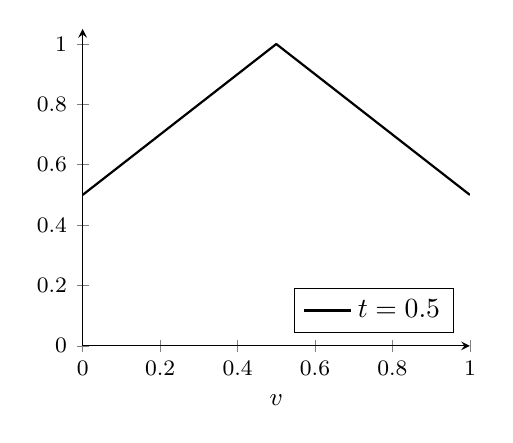
\begin{tikzpicture}
			\pgfplotsset{every axis legend/.append style={at={(0.96,0.04)},anchor=south east}}
			\begin{axis}[small,xlabel=$v$,xmin=0,xmax=1.0,ymin=0.0,ymax=1.05,axis lines=left]
				\addplot[thick,black,domain=0.0:1.0,samples=500]
					{ 1.0 - abs(0.5 - x)/1.0
};
				\addlegendentry{$t=0.5$}
			\end{axis}
		\end{tikzpicture}
		}
		\caption{$\mathsf{sim_\text{dist}}$}
		\label{fig:kappa-simdistplot}
	\end{subfigure}%
	\begin{subfigure}[b]{0.33\linewidth}
		\centering
		\resizebox{\linewidth}{!}{
		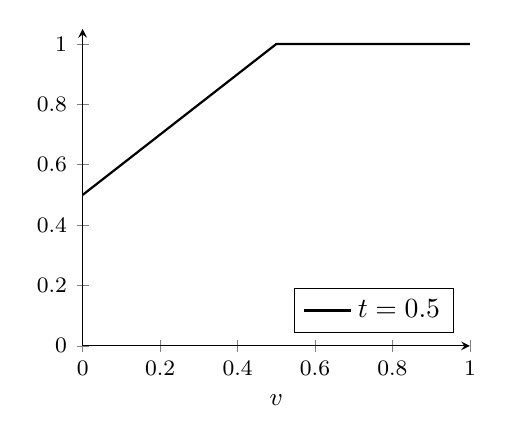
\begin{tikzpicture}
			\pgfplotsset{every axis legend/.append style={at={(0.96,0.04)},anchor=south east}}
			\begin{axis}[small,xlabel=$v$,xmin=0,xmax=1.0,ymin=0.0,ymax=1.05,axis lines=left]
				\addplot[thick,black]
					coordinates {
						(0.0,0.5)
						(0.5,1.0)
						(1.0,1.0)
					};
			\addlegendentry{$t=0.5$}
			\end{axis}
		\end{tikzpicture}
		}
		\caption{$\mathsf{sim_\text{asym}}$}
		\label{fig:kappa-simasymplot}
	\end{subfigure}%
	\begin{subfigure}[b]{0.33\linewidth}
		\centering
		\resizebox{\linewidth}{!}{
		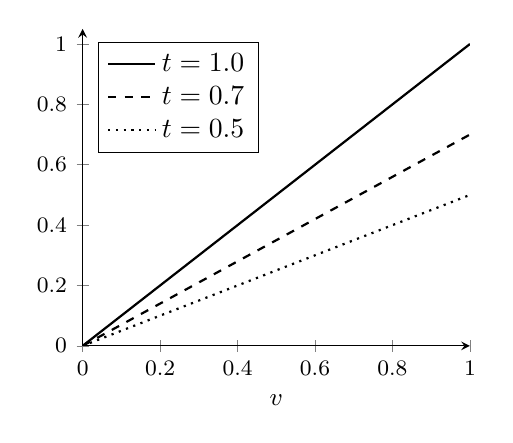
\begin{tikzpicture}
			\pgfplotsset{every axis legend/.append style={at={(0.04,0.96)},anchor=north west}}
			\begin{axis}[small,xlabel=$v$,xmin=0,xmax=1.0,ymin=0.0,ymax=1.05,axis lines=left]
				\addplot[thick,black,domain=0.0:1.0,samples=500]
					{ 1.0 * x
};
				\addlegendentry{$t=1.0$}
				\addplot[dashed,thick,black,domain=0.0:1.0,samples=500]
					{ 0.7 * x
};
	
				\addlegendentry{$t=0.7$}
				\addplot[dotted,thick,black,domain=0.0:1.0,samples=500]
					{ 0.5 * x
};
				\addlegendentry{$t=0.5$}
			\end{axis}
		\end{tikzpicture}
		}
		\caption{$\mathsf{sim_\text{score}}$}
		\label{fig:kappa-simscoreplot}
	\end{subfigure}%
	\caption{Similarity metrics plotted as a function of the value $v$, for different similarity functions. The y-axis is the output from the similarity function, the target value $t$ is given in the legend of each line.}
	\label{fig:kappa-similarityfunctions}
\end{figure}

\subsubsection{Hybrid Recommender Systems}
\label{sec:kappa-hybridrecommenders}

Each of the three classes of recommender systems mentioned before has their own advantages and disadvantages.
Knowledge-based systems works well in a cold-start setting, but does not consider user history.
Content-based systems works well when new items are added, but fails to present recommendations for new users.
Collaborative filtering methods can utilize ratings from other users, but may not work well if the rating matrix is too sparse.

The idea of hybrid recommenders is to combine several recommender methods, such that they do not run in isolation, but rather together with other methods.
This allows the hybrid recommender to benefit from the advantages of the individual recommender methods, and hopefully avoid the disadvantages.

Hybrid recommenders can be constructed in various ways, depending on how the different subsystems are interconnected, what input each subsystem has, and how the output is constructed.
Examples of constructions as well a classifications are described in \cite{burke:2002}, however, we will only focus on one particular construction, which is described next.

One straightforward way to construct a hybrid recommender is to construct a \emph{weighted} hybrid, which has a layout as in Figure~\ref{fig:kappa-weightedhybrid}.
Each subsystem has the same input, and the output is then calculated as a weighted average where each individual subsystem has a certain weight $w_i$.
We will later return to this type of hybrid recommender when we construct a recommender system in \paperref{ch:recsys}.

\begin{figure}[th]
	\centering
	\begin{tikzpicture}[scale=1, every node/.style={scale=1}, node distance=1cm, font=\small\sffamily]
		\node[draw]                       (recommender1) {Recommender 1};
		\node[draw,below=of recommender1] (recommender2) {Recommender 2};
		\node[draw,below=of recommender2] (recommendern) {Recommender $n$};
		\node[] at ($(recommender2)!0.5!(recommendern)$) {\ldots};
		
		\node[draw,right=of recommender2,align=center] (combiner) {Weighted\\average};
		
		\node[left=of recommender2]  (input)           {Input};
		\node[right=of combiner]     (recommendations) {Recommendations};
		
		\coordinate (recommendernshifted) at ([yshift=-0.5cm]recommendern.south east);
		\draw[dashed] ([xshift=-0.5cm,yshift=+0.5cm]recommender1.north west) rectangle ([xshift=+0.5cm]combiner.east |- recommendernshifted);
		
		\draw[->] (input) -- (recommender1.west);
		\draw[->] (input) -- (recommender2.west);
		\draw[->] (input) -- (recommendern.west);
		
		\draw[->] (recommender1.east) -- node[above] {$w_1$} (combiner);
		\draw[->] (recommender2.east) -- node[above] {$w_2$} (combiner);
		\draw[->] (recommendern.east) -- node[below,outer sep=3pt] {$w_n$} (combiner);
		
		\draw[->] (combiner) -- (recommendations);
	\end{tikzpicture}
	\caption{Overview of a weighted recommender system}
	\label{fig:kappa-weightedhybrid}
\end{figure}

\subsection{Research on Recommender Systems}
% was Recommender Systems in Software Security

Research in recommender systems can be made in several different ways.
Focus can be on presenting new or refined algorithms for the various recommender methods, as well as introducing new use cases of recommender systems.

Significant advances, specifically in the area of collaborative filtering, have been made during the course of the Netflix Prize \cite{netflixprize}.
The competition, organized by the media-services provider Netflix, took place from October 2006 until the winning team was announced in September 2009.
The prize awarded to the winner was 1 million US dollars, if the accuracy of the designed solution beat Netflix's own recommender Cinematch by 10\%.
Together with the announcement of the competition, Netflix also published a large dataset of anonymized user rankings useful for training recommenders.
The winning recommender, named ``BellKor's Pragmatic Chaos'', from the combination of solutions from three different teams, finally achieved an improvement of 10.06\%.
The design is described in three separate papers \cite{koren:2009,toscher:2009,piotte:2009}.
For other contributions related to the prize refer to, e.g., \cite{zhou:2008,takacs:2008} for some examples of systems using the anonymized dataset.

Research is also focused on applying recommender systems in new areas to find use~cases that have not yet seen the potential benefits of recommender systems.
Some examples of use~cases for recommenders include movie recommendations \cite{diao:2014,harper:2015}, e-commerce \cite{huang:2007,castroschez:2011}, music \cite{schedl:2015,kaminskas:2013}, web services \cite{zheng:2009}, or research articles \cite{wang:2018}.

In this dissertation, we consider the application of recommender systems in the cyber security domain.
The subject of cyber security is wide, and recommender systems have been proposed to several different areas.
Previous work in the area includes the use or recommender systems to
recommend cyber defence actions to cyber warriors \cite{lyons:2014},
detect unsafe coding practices and suggest fixes in Java source code \cite{nembhard:2019},
and predict attacks in a network using a graph of attack paths \cite{polatidis:2017}.

More specifically, the use of recommender systems can also be applied to the area of software vulnerability management.
As new software vulnerabilities are discovered, it is increasingly important for software vendors to discover, analyse, and handle them.
Vulnerabilities can arise both in code developed by the vendors themselves, but can also be discovered in third-party libraries included in the software package.
Using a recommender system to aid in various parts of the vulnerability management life cycle has been proposed in earlier work.
In \cite{farris:2018} the authors propose a recommender system to reduce time-to-vulnerability remediation as well as total vulnerability exposure within an organization.
Others have instead looked at using recommender systems to propose actions to take after discovering a vulnerability \cite{gadepally:2016}.
Text-mining is used in \cite{lee:2018} to find vulnerabilities related to each other, which is then used to construct a vulnerability ranking.

In \paperref{ch:recsys} we also construct a recommender system for vulnerabilities.
Our recommender is based on a hybrid approach (see Section~\ref{sec:kappa-hybridrecommenders}) and the goal is to produce a user-specific vulnerability scoring.
This is in contrast to common vulnerability scoring methods such as CVSS \cite{cvss2spec,cvss3spec} used by NVD \cite{nvd} to provide a non-individualized vulnerability score.
This recommendations are generated by combining traits from two of the previously mentioned recommender types, knowledge-based, and content-based, combined with domain-specific knowledge of the field of software vulnerabilities.

\subsection{Privacy in Recommender Systems}
\label{sec:kappa-recsysprivacy}

After discussing how recommenders can be used to aid in software security, we now turn the focus to security of the recommender systems themselves.
For recommenders to provide useful output to users, they clearly must store and process information about every user of the system.
Such data collection gives rise to privacy concerns, since the data can be used to build an intimate profile of a user's interests, opinions, identity, or other personal information, depending on the type of recommender.

Earlier research has shown that the privacy risks of recommenders exists in real life.
In \cite{narayanan:2008}, the authors present a de-anonymization attack on the Netflix Prize dataset.
While anonymization techniques had been applied to the dataset before being published by Netflix, the authors show that with knowledge of some information about a user, their full record can be identified in the dataset.
Applied to the Netflix dataset, this means that knowing some information about a user's previously watched or rated movies, could allow an attacker to gain information about all movies the user has watched or rated.

By using differential privacy \cite{dwork:2006}, the authors of \cite{mcsherry:2009} present a design that builds privacy into recommender systems.
They apply differential privacy to the recommenders, while still maintaining a high accuracy despite the introduced noise.

Potential privacy risks of collaborative filtering are also discussed in \cite{calandrino:2011}, where the authors present inference attacks to get customer data by observing public output from recommender system.
Such risks are also one reason why collaborative filtering methods are avoided in some settings, for example in the recommender system presented in \paperref{ch:recsys} of this dissertation.
Privacy-preserving methods for collaborative filtering tries to solve this, but are not covered further in this dissertation, instead we refer to previous work in the area, e.g., \cite{zhan:2010,polat:2003,canny:2002,parameswaran:2007,polat:2005}.

In this dissertation, \paperref{ch:recsyssgx} presents a privacy-preserving system to provide recommendations for software vulnerabilities.
The user profiles contain sensitive information, since they can provide an observer with information about internal vulnerability management processes of the user.
By using trusted computing, specifically Intel SGX (see Section~\ref{sec:kappa-sgx}), and k-anonymity \cite{samarati:1998,samarati:2001}, we propose a solution that preserves the privacy of the user profiles, without requiring modification of the recommender system itself.

\newpage
\section{Cryptography}
\label{sec:kappa-cryptography}

The area of cryptography covers a wide range of different functionality, e.g., making messages unreadable to unauthorized parties, ensuring that they have not been modified during transfer, and creating digital signatures to provide proof of authenticity.
The different algorithms that provide this functionality can be classified into different categories, called cryptographic primitives.
Common cryptographic primitives include one-way hash functions, symmetric encryption algorithms, public-key encryption algorithms, and digital signatures.
Such primitives are commonly combined into cryptographic protocols, which provide a richer set of features.
An example of such a protocol is Transport Layer Security (TLS) \cite{rfc8446}, which provides a secure channel with confidentiality, integrity, and authentication.
TLS achieves this by combining cryptographic primitives such as encryption algorithms, and key exchange protocols.

The purpose of encryption algorithms -- commonly called \emph{ciphers} -- is to conceal messages such that they are unintelligible to an unauthorized party.
Only an authorized party can reverse the steps of the encryption -- called decryption -- and retrieve the original message.
An overview of the process can be seen in Figure~\ref{fig:kappa-encdec}.
A message $m$, also called \emph{plaintext}, is sent into the encryption algorithm together with a key $K_e$.
The resulting encrypted message $c$, called \emph{ciphertext}, is the result from this encryption step.
On the receiver's end, the ciphertext is fed into the decryption algorithm, together with a key $K_d$.
The output from the decryption is the original message $m$.
This description is very general, and applicable to ciphers in general.

\begin{figure}[ht]
	\centering
	\begin{tikzpicture}[scale=1, every node/.style={scale=1}, node distance=2cm, font=\small\sffamily]
		\node[draw]                (encryption)  {Encryption};
		\node[left of=encryption]  (plaintext)   {$m$};
		\node[right of=encryption] (ciphertext)  {$c$};
		\node[below=0.5cm of encryption] (key-e) {$K_e$};
		
		\draw[->] (plaintext.east) -- (encryption.west);
		\draw[->] (encryption.east) -- (ciphertext.west);
		\draw[->] (key-e.north) -- (encryption.south);

		\node[right of=ciphertext,draw]  (decryption)   {Decryption};
		\node[right of=decryption]        (plaintext2)   {$m$};
		\node[below=0.5cm of decryption] (key-d)        {$K_d$};
		
		\draw[->] (ciphertext.east) -- (decryption.west);
		\draw[->] (decryption.east) -- (plaintext2.west);
		\draw[->] (key-d.north) -- (decryption.south);
	\end{tikzpicture}
	\caption{Overview of encryption and decryption flow}
	\label{fig:kappa-encdec}
\end{figure}

Ciphers can be divided into two categories, depending on how the keys $K_e$ and $K_d$ are related.
In asymmetric ciphers, or public-key ciphers, $K_e$ and $K_d$ are different, but mathematically related.
One of the keys is kept secret, and is called the \emph{private key}, while the other key is made public for everyone, and is called the \emph{public key}, thus giving the alternative name public-key cipher.
An important requirement is that knowing the public key $K_e$ should not help anyone calculate the private key $K_d$.
This allows the public key to be distributed freely, while $K_d$ should be kept private.

In an encryption setting, the public key is $K_e$, and thus anyone can encrypt messages to a certain recipient.
While anyone can encrypt messages, only the user in possession of the private key $K_d$ can decrypt the received ciphertexts.
Well-known asymmetric ciphers include RSA \cite{rivest:1978}, which can also be used to create digital signatures.
Asymmetric cryptography will not be covered in more detail in this dissertation, for more details refer to \cite{smart:2016}, and instead we shift focus to symmetric ciphers.

\subsection{Symmetric Ciphers}

If a shared key is used for both encryption and decryption, the cipher is called \emph{symmetric}.
While common, it is not a strict requirement for $K_e = K_d$ in symmetric ciphers; the keys can also be different but closely linked, such that knowledge of $K_e$ means that $K_d$ can be easily calculated, and vice versa \cite{smart:2016}.
For the remainder of this dissertation, we assume that $K_e = K_d = K$ when discussing symmetric ciphers.

Symmetric ciphers require the sender and receiver to first agree on a shared key $K$, and then to keep this key secret, since anyone with access to the key can decrypt ciphertexts.
Symmetric ciphers can be designed in multiple ways, and can in turn be classified into two categories: block ciphers and stream ciphers.

An overview of a block cipher can be seen in Figure~\ref{fig:kappa-blockcipher}.
\begin{figure}[ht]
	\centering
	\begin{tikzpicture}[scale=1, every node/.style={scale=1}, node distance=2cm, font=\small\sffamily]
		\node[draw,align=center]     (encryption)  {Block cipher\\encryption};
		\node[left of=encryption]  (plaintext)   {$m_i$};
		\node[right of=encryption] (ciphertext)  {$c_i$};
		\node[below=0.5cm of encryption] (key-e) {$K$};
		
		\draw[->] (plaintext.east) -- (encryption.west);
		\draw[->] (encryption.east) -- (ciphertext.west);
		\draw[->] (key-e.north) -- (encryption.south);
	\end{tikzpicture}
	\caption{Encryption of a plaintext block with a block cipher}
	\label{fig:kappa-blockcipher}
\end{figure}
The differences from the general description of a cipher from Figure~\ref{fig:kappa-encdec} earlier are that the key is symmetric, and thus denoted simply by $K$, and that the plaintext and ciphertext are divided into \emph{blocks} of fixed size.
One block of the message $m$ is denoted $m_i$, and the same is true for the ciphertext blocks $c_i$.
A block cipher is a permutation from the plaintext space to the ciphertext space, but the permutation depends on the key $K$, such that knowledge of $K$ is required to map a block $m_i$ to $c_i$, and vice versa.
Worth noting is that to use a block cipher, it must be combined with a \emph{mode of operation}, which uses the block cipher as a building block.
For an in depth discussion about block ciphers and modes of operation refer to \cite{smart:2016}.
Instead, we now move on to stream ciphers.

\subsection{Stream Ciphers} \label{sec:kappa-streamciphers}

A stream cipher is a symmetric cipher that works on a stream of symbols.
The cipher generates a keystream, commonly denoted by $z$, which is used both to encrypt a message, and to decrypt a corresponding ciphertext.
The keystream is a pseudo-random stream of symbols generated by providing a key $K$ and public initialization vector $IV$ to the cipher.

Encryption is performed by combining the keystream with the plaintext using an output function $h$ as
\begin{equation} \label{eq:kappa-streamcipherencrypt}
	c_i = h(m_i, z_i) \,,
\end{equation}
where $c_i$, $m_i$, and $z_i$ are the $i^{\text{th}}$ symbol of the ciphertext, message, and keystream, respectively.
In a similar way, decryption is performed by
\begin{equation} \label{eq:kappa-streamcipherdecrypt}
	m_i = h^{-1}(c_i, z_i) \,.
\end{equation}

There are two main categories of stream ciphers, which differ in the way the keystream $z$ is constructed: \emph{synchronous} and \emph{self-synchronizing} stream ciphers.
The main difference is that synchronous stream ciphers generate keystream using only key and IV, while in self-synchronizing stream ciphers, the keystream also depends on previous ciphertext symbols.
The most common type is the synchronous stream cipher, which will be described in more detail below.

The general design of a synchronous stream cipher can be seen in Figure~\ref{fig:kappa-syncstreamcipher}.
\begin{figure}[ht]
	\centering
	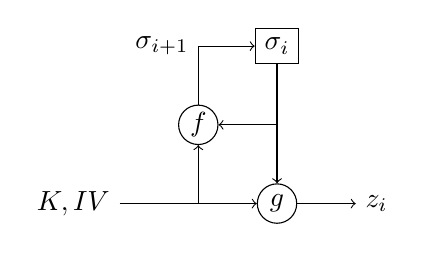
\begin{tikzpicture}[scale=1, every node/.style={scale=1}, node distance=1cm]
		\node[draw,circle,align=left,inner sep=0pt,minimum size=0.5cm]     (g)  {$g$};
		\node[right of=g,anchor=west] (z) {$z_i$};
		\coordinate[left of=g]  (kgmiddle);
		\node[left of=kgmiddle,anchor=east] (k)    {$K, IV$};
		\coordinate[above of=g] (sigmagmiddle);
		\node[draw,circle,inner sep=0pt,minimum size=0.5cm] (f) at (kgmiddle |- sigmagmiddle) {$f$};
		\node[draw,above of=sigmagmiddle] (sigma) {$\sigma_i$};
				
		\draw[->] (k) -- (kgmiddle) -- (f);
		\draw[->] (kgmiddle) -- (g);
		
		\draw[->] (sigma) -- (sigmagmiddle) -- (g);
		\draw[->] (sigmagmiddle) -- (f);
		
		\draw[->] (f) |- node[left] {$\sigma_{i+1}$} (sigma);
		
		\draw[->] (g) -- (z);
	\end{tikzpicture}
	\caption{A general figure of a synchronous stream cipher, taking key and IV as input, and outputting keystream}
	\label{fig:kappa-syncstreamcipher}
\end{figure}
The cipher has an internal state $\sigma$ which for every symbol $i$ is updated to the next state $\sigma_{i+1}$ by the next-state function $f$, which can depend on the key, IV, and current state $\sigma_i$.
For every symbol, the function $g$ calculates the current keystream symbol $z_i$, which depends on the current state $\sigma_i$, the key, and the IV.
Finally, as in (\ref{eq:kappa-streamcipherencrypt}) and (\ref{eq:kappa-streamcipherdecrypt}), the keystream is combined with the plaintext or ciphertext to perform encryption or decryption, respectively.
Stream ciphers generally also have an \emph{initialization phase}, performed before the ciphers start to generate actual keystream.
The initialization phase is not shown in Figure~\ref{fig:kappa-syncstreamcipher}, but will be discussed in more detail later in Section~\ref{sec:kappa-streamcipherinitialization}.

The most common design of synchronous stream ciphers is the \emph{binary additive stream cipher}.
This design has the following properties:
\begin{itemize}
	\item Each plaintext, ciphertext, and keystream symbol is a binary digit.
	\item The output function $h$ is the logical exclusive or operation (XOR), hereafter denoted $\oplus$.
\end{itemize}
Thus, encryption of a plaintext bit $m_i$ and decryption of a ciphertext bit $c_i$ is made with the output functions
\begin{align}
	h(m_i, z_i) &= m_i \oplus z_i        \label{eq:kappa-additiveencrypt} \\
	h^{-1}(c_i, z_i) &= c_i \oplus z_i   \label{eq:kappa-additivedecrypt}
\end{align}
using the keystream bit $z_i$.
We can easily show that this works since

\begin{equation}
	h^{-1}( h(m_i, z_i), z_i) = m_i \oplus z_i \oplus z_i = m_i \,.
\end{equation}
It is worth noting that this is a design where encryption and decryption are done in the same way -- avoiding the need for separate implementations of encryption and decryption, which is the case for some block cipher modes of operation, e.g., CBC mode.

The binary additive stream cipher above mimics another well-known cryptosystem called the \emph{one-time pad}.
In a one-time pad, each keystream symbol $z_i$ is independently and randomly generated, and then added to the plaintext just as in (\ref{eq:kappa-additiveencrypt}).
Furthermore, such a keystream must only be used \emph{once} -- giving the cryptosystem its name -- which also implies that the keystream much be at least as long as the plaintext.
While such a system may be inconvenient due to the large keystream that needs to be distributed, it has an extremely strong security guarantee, it is \emph{unconditionally secure}.
Next, we describe this and several other definitions of security.

\subsection{Security}

What does it mean for a cipher to be secure?
Indeed, there are several different definitions of what security means in this context.
While the terminology may differ slightly in the field of cryptography, these are the definitions used throughout this dissertation.

\subsubsection{Unconditional Security}

Unconditional security, or information-theoretic security, means that an adversary cannot break the cryptosystem, even with unlimited computing power.
As described earlier, the one-time pad is an example of such a system.

\subsubsection{Provable Security}

In some cases, it may be possible to base a cryptosystem on a problem that is thought to be hard.
If it is possible to prove that breaking the cryptosystem is related to solving some other well-known hard problem, the cryptosystem is said to by provably secure.
This is especially common in asymmetric cryptography, where many cryptosystems are designed to be related to well-known mathematical problems that are hard to solve.

An example of such a system with a corresponding problem is RSA \cite{rivest:1978}, which is based on the RSA problem, which can be stated as: Given a ciphertext $c$, and $e$ such that $\gcd(e, \phi(N)) = 1$, find the plaintext $m$ such that $m^e = c \mod N$.

\subsubsection{Empirical Security}
A weaker assumption is that of empirical security.
A cipher is empirically secure if empirical methods have been used to design and analyse it.
The rationale behind calling it secure is this: if a cipher has been thoroughly analysed during some longer time frame, without any attacks being found, it can be seen as secure.
While the approach is pragmatic, there are no formal proofs for security, and a new attack may be found in the future.

\subsection{Attacks}

Given that the whole purpose of a cipher is to conceal valuable information from an adversary, it is only natural that ciphers are under attack from both adversaries, as well as those wanting to select a cipher to protect their own information.
Attacks come in many forms, and can be categorized depending on their properties.
In this section, a few different kind of attacks and attack models will be described, with focus on those that are relevant for this dissertation.

\subsubsection{Key-recovery Attacks}

The goal of a key-recovery attack is simple: to gain access to the secret key $K$.
Knowledge of the key allows an adversary to decrypt ciphertexts.

\subsubsection{State-recovery}

In a state-recovery attack, the goal is to recover the internal state of the cipher.
In the case of a stream cipher, knowing the internal state at time $t$ may allow an attacker to construct a valid keystream from time $t$ and forward, which can be used to decrypt ciphertexts.
Depending on the cipher, it may also be possible to calculate earlier keystream bits, if the next-state function $f$ is invertible.
In addition, if both the next-state function $f$ \emph{and} the initialization phase is invertible, the key can be recovered, thus turning into a key-recovery attack.

\subsubsection{Distinguishers}

In a distinguishing attack, the goal for the attacker is to determine if a sequence of symbols comes from a stream cipher, or is just random data.
Consider the scenario in Figure~\ref{fig:kappa-distinguisher}.
\begin{figure}[ht]
	\centering
	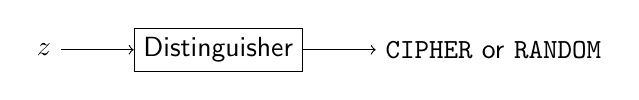
\begin{tikzpicture}[scale=1, every node/.style={scale=1}, node distance=2cm, font=\sffamily]
		\node[draw]     (distinguisher)  {Distinguisher};
		\node[left of=distinguisher,anchor=east] (keystream) {$z$};
		\node[right of=distinguisher,anchor=west] (result) {\texttt{CIPHER} or \texttt{RANDOM}};
		
		\draw[->] (keystream) -- (distinguisher);
		\draw[->] (distinguisher) -- (result);
	\end{tikzpicture}
	\caption{A distinguisher taking keystream $z$ as input, and outputting a decision}
	\label{fig:kappa-distinguisher}
\end{figure}
The goal of the distinguisher is to determine if the given keystream $z$ is produced by a cipher, or if it is just random data.
Naturally, for a given keystream, the distinguisher can always guess the correct answer with a probability of 0.5, simply by picking \texttt{RANDOM} or \texttt{CIPHER} uniformly random.
Thus a distinguishing attack is only considered successful if the distinguisher can guess the result with a higher probability compared to a uniformly random guess.
While the attack is not as strong as for example a key-recovery attack, it is still useful in a number of settings.
First, it may be possible to use the distinguisher as a part of a key-recovery attack, as done in \cite{englund:2005} and \cite{hell:2007}.
Second, if an adversary knows that a ciphertext is the encryption of one of two possible plaintexts, their respective keystreams can be derived, and passed through the distinguisher to determine which of the two plaintexts that were likely sent.
Third, the distinguisher is a useful tool in the design of stream ciphers, since the keystream from a well-designed cipher should appear random to an outside observer without the key.
This third and final use case is discussed in more detail next.

\subsection{Stream Cipher Initialization and Design}
\label{sec:kappa-streamcipherinitialization}

In Section~\ref{sec:kappa-streamciphers}, an overview of synchronous stream ciphers is given, describing the internals of the cipher and how keystream is generated.
Recall that the IV is public, and easily accessible to an attacker, thus it is important that knowledge of the IV does not allow an attacker to gain information about the keystream.
To prevent this, ciphers can mix IV and key bits during an \emph{initialization phase}, before the cipher starts to output actual keystream symbols.

One possible way to perform initialization is to repeatedly apply the next-state function $f$ \emph{before} the cipher starts to generate keystream.
Each such repeated application of the update function $f$ is called a \emph{round}.
This approach is shown in Figure~\ref{fig:kappa-cipherinitialization}.
\begin{figure}[ht]
	\centering
	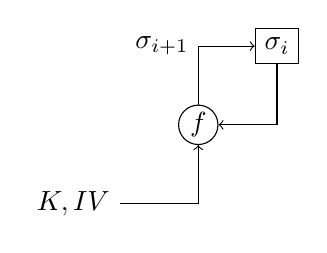
\begin{tikzpicture}[scale=1, every node/.style={scale=1}, node distance=1cm]
	\node[circle,align=left,inner sep=0pt,minimum size=0.5cm]     (g)  {};
	\coordinate[left of=g]  (kgmiddle);
	\node[left of=kgmiddle,anchor=east] (k)    {$K, IV$};
	\coordinate[above of=g] (sigmagmiddle);
	\node[draw,circle,inner sep=0pt,minimum size=0.5cm] (f) at (kgmiddle |- sigmagmiddle) {$f$};
	\node[draw,above of=sigmagmiddle] (sigma) {$\sigma_i$};
	
	\draw[->] (k) -- (kgmiddle) -- (f);
	\draw[->] (sigma) |- (f);
	
	\draw[->] (f) |- node[left] {$\sigma_{i+1}$} (sigma);
	\end{tikzpicture}
	\caption{One way to perform the initialization phase by repeatedly applying the next-state function $f$ to update the state $\sigma_i$}
	\label{fig:kappa-cipherinitialization}
\end{figure}
The initialization phase typically consist of a number of such initialization rounds, and an important part of designing the cipher is to select a suitable amount of rounds.
If too many rounds are performed, the performance of the cipher will suffer, since there is an increased delay before the cipher can start to output actual keystream.
On the other hand, if too few rounds are used, it may be possible to attack the cipher since the mixing of key and IV bits is insufficient.

To try to find such insufficient mixing, a chosen-IV attack can be performed.
As the name implies, in this setting the attacker can freely modify the IV of the cipher.
One way to perform such an attack is to look at certain keystream bits, and analyse the algebraic structure of such a bit.
One such attack was performed in \cite{saarinen:2006}, in which Saarinen used the $d$-Monomial test introduced by \cite{filiol:2002} to analyse the algebraic normal form (ANF) of certain keystream bits.

A Boolean function of $b$ variables, $f \colon \mathbb{F}_2^b \to \mathbb{F}_2$, can be written on ANF, which has the following structure:
\begin{align*}
	f(x_1, \ldots, x_b) = c_0 \oplus c_1 x_1 \oplus \ldots \oplus c_b x_b \oplus c_{b+1} x_1 x_2 \oplus \ldots \oplus c_m x_1 x_2 \ldots x_b \,,
\end{align*}
where the coefficients $c_i \in \mathbb{F}_2$ describe if the term is included in the ANF or not.
The ANF consists of up to $2^b$ monomials, with an average of $2^{b-1}$ monomials in a random Boolean function $f$.
Furthermore, if $k$ is the degree of such a monomial ($0 \le k \le b$), the ANF has on average $\frac{1}{2} {\binom{b}{k}}$ monomials of degree $k$.
The reader is referred to \cite{filiol:2002} for proofs.

The previously mentioned average monomial count can be used to perform statistical tests.
In \cite{saarinen:2006}, the $\chi^2$ test is used to analyse if the Boolean functions of the ciphers' keystream bits are biased, for monomials up to degree $d=4$.

A similar approach was presented in \cite{englund:2007}, where the $d$-Monomial test is replaced with a Maximum Degree Monomial (MDM) test, where only the monomial of the highest degree is considered, i.e., $d=b$.
The rationale behind this approach is that the maximum degree monomial is only likely to exist in the ANF if there has been sufficient mixing of the IV bits.
Furthermore, finding the coefficient $c_m$ of the maximum degree monomial can be done simply by calculating $c_m$ as:
\begin{align}
	c_m = \bigoplus_{\bm{x} \in \mathbb{F}^b_2}^{} f(\bm{x}) \,.
\end{align}

In this context, it is also relevant to mention AIDA and Cube Attacks, introduced in \cite{vielhaber:2007} and \cite{dinur:2009}, respectively.
These attacks are key-recovery attacks, thus trying to derive the secret key of the cipher.
In both papers modified versions of the cipher Trivium \cite{canniere:2006} are attacked, where the modifications consist of reducing the number of initialization rounds.

A property shared between \cite{saarinen:2006,englund:2007,vielhaber:2007,dinur:2009} is that they work on a \emph{subset} of IV bits.
The selection of this subset is a problem in itself, since it affects the outcome of the attack.
In \cite{stankovski:2010}, \citeauthor{stankovski:2010} considers this problem and presents a greedy, iterative, algorithm to find subsets of increasingly large sizes.
In addition, subsets of both IV and key bits are considered.
The author also defines the \emph{MDM signature}, which is used as a metric in the greedy algorithm.
The MDM signature is based on the MDM test described above; recall that the coefficient of the maximum degree monomial can be found by summing over all entries in the truth table.
In the MDM signature this is extended, so instead of looking at a single coefficient from the cipher's first keystream bit, the output from the (normally suppressed) initialization phase is considered instead.
Thus, if a cipher has $l$ initialization rounds, the MDM signature will consist of $l$ coefficients, each one corresponding to the coefficient of the maximum degree monomial of that particular output bit, giving a signature on the following form:
\begin{align}
	\underbrace{0000000111010110\ldots101}_{l\text{ coefficients}} \,.
\end{align}

The idea of this metric is that the lack of ones in the beginning of the MDM signature corresponds to an insufficient mixing of IV bits in the cipher, since the  maximum degree monomial has not yet been seen.

However, since finding the MDM coefficients requires summing over all entries in the truth table, it is infeasible to consider all Boolean input bits, since this would correspond to $2^b$ invocations, where $b=128$ or even more for modern ciphers.
Instead, the author tries to maximize the number of initial zeros in the MDM signature, and greedily adds more IV bits to the subset to maximize this metric.

In \paperref{ch:slightlygreedy}, we consider precisely this problem of finding subsets for attacks such as those described earlier.
While \cite{stankovski:2010} selected the subsets in a greedy fashion, we propose a generalized version, finding better subsets.
The main observation is that greedy algorithms risk getting stuck in local optima, which our generalized algorithm avoids by keeping a list of several good candidates from previous iterations.
Furthermore, the algorithm can add more than one bit in each iteration, at the expense of higher computational complexity.

Further work in the area has been done in \cite{yang:2019}, where a new algorithm is proposed, building upon the work in \paperref{ch:slightlygreedy}.
Instead of requiring the summation of all possible IV combinations (thus having a complexity of $\mathcal{O}(2^n)$ for a subset of size $n$), the authors use an algorithm to estimate the degree of the monomial instead.
This allows them to find larger subsets with lower computational complexity.

\chapter{Contributions and Conclusions}

This dissertation has focused on different preventive measures in the area of cyber security.
The different contributions can be visualized within the area as in Figure~\ref{fig:kappa-contributions}, where only preventive measures that have been covered in this dissertation are included.
After this, the contributions are described in more detail in Section~\ref{sec:kappa-contributions}, followed by conclusions in Section~\ref{sec:kappa-conclusions}.

\begin{figure}[ht]
	\centering
	\begin{tikzpicture}[scale=1.0, every node/.style={scale=1.0,font=\sffamily}, node distance=2cm,
			area/.style={draw,dotted,ellipse,font=\small\sffamily},
			label/.style={align=center,font=\small\sffamily},
			paper/.style={draw,fill=black,minimum width=0.15cm,minimum height=0.15cm,inner sep=0pt},
			paperlabel/.style={font=\footnotesize\sffamily\itshape}]
		
		\node[draw,dashed,ellipse,minimum width=12cm,minimum height=8cm] (preventive) at (0,0) {};
		\node[below=0.5cm of preventive.north] {Preventive measures};
		
		\node[area,minimum width=5cm,minimum height=5cm,anchor=west,right=0.5cm of preventive.west] (tc) {};
		\node[label,below=0.5cm of tc.north] {Trusted computing};
		
		\node[area,minimum width=3cm,minimum height=3cm,anchor=east,left=0.5cm of preventive.east] (crypto) {};
		\node[label,below=0.5cm of crypto.north] {Cryptography};
		
		\node[area,minimum width=4cm,minimum height=4cm,anchor=east,above=0.5cm of preventive.south] (vuln) {};
		\node[label,above=0.3cm of vuln.south] {Vulnerability\\assessment};
		
		% The paper coordinates
		
		\node[paper,above left=1.0cm and 0.9cm of tc.center] (paperI) {};
		\node[paper,above right=1.0cm and 0.1cm of tc.center] (paperII) {};
		\node[paper,below left=0.4cm and 0.2cm of tc.center] (paperIII) {};
		\node[paper,above right=1.2cm and 0.9cm of vuln.center] (paperIV) {};
		\node[paper] (paperV) at ($(vuln.north west)!0.5!(tc.south east)$) {};
		\node[paper,below=0.0cm of crypto.center] (paperVI) {};
		
		% Paper labels and arrows
		\node[paperlabel,below left=0.5cm and 0.3cm of paperI] (paperIlabel) {\paperref{ch:tpmhas}};
		\node[paperlabel,below right=0.1cm and 0.5cm of paperII] (paperIIlabel) {\paperref{ch:tpm12to20}};
		\node[paperlabel,below left=0.4cm and 0.5cm of paperIII] (paperIIIlabel) {\paperref{ch:trustanchors}};
		\node[paperlabel,below right=0.5cm and 0.5cm of paperV] (paperVlabel) {\paperref{ch:recsyssgx}};
		\node[paperlabel,below=0.5cm of paperIV] (paperIVlabel) {\paperref{ch:recsys}};
		\node[paperlabel,below=0.5cm of paperVI] (paperVIlabel) {\paperref{ch:slightlygreedy}};
		
		\draw[->] (paperIlabel)   -- (paperI);
		\draw[->] (paperIIlabel)  -- (paperII);
		\draw[->] (paperIIIlabel) -- (paperIII);
		\draw[->] (paperIVlabel)  -- (paperIV);
		\draw[->] (paperVlabel)   -- (paperV);
		\draw[->] (paperVIlabel)  -- (paperVI);
	\end{tikzpicture}
	\caption{The different contributions of this dissertation to the area of preventive measures in cyber security. Each paper is positioned according to the area (or areas) it contributes to.}
	\label{fig:kappa-contributions}
\end{figure}


\section{Contributions}
\label{sec:kappa-contributions}

In this section the main contributions of this dissertation are described.
To give a quick overview, the contributions are:

\begin{itemize}
  \item A way of using TPM secure storage in high availability systems (\paperref{ch:tpmhas}), where we describe a use case where the TPM is used to store key material in a high availability system, consisting of multiple independent Computational Units (CUs) for availability purposes.
  The secure storage must be duplicated on each individual CU for availability purposes, and we describe a solution for this, supporting both TPM 1.2 and TPM 2.0.

  \item The migration of keys from TPM 1.2 to TPM 2.0, while still retaining behaviour with regard to, e.g., authorization, PCR values, and migration, even though the TPM 2.0 standard is not backwards-compatible by design (\paperref{ch:tpm12to20}).
  The proposed design utilizes new features of TPM 2.0 to achieve the behaviour of TPM 1.2.

  \item A design to protect core assets and enrollment of network security elements used in Softward Defined Networking (SDN) entities (\paperref{ch:trustanchors}).
  We describe both a way to protect core assets such as credentials by using isolated execution environments, and also a mechanism to perform secure enrollment of entities into the SDN by using remote attestation.

  \item A recommender system that generates user-specific scorings for software vulnerabilities (\paperref{ch:recsys}).
  The system takes explicit user preferences into account, together with information learned from previous interactions with the system, and creates a user profile.
  The profile is then used to generate a vulnerability scoring that is customized to the user, as opposed to other severity metrics such as the CVSS score.

  \item A privacy-preserving mechanism that can be used to protect the client profile in recommender systems for software vulnerabilities (\paperref{ch:recsyssgx}).
  Such profiles contain information about how clients have interacted with previous software vulnerabilities, as well as client preferences about vulnerability properties, which may be undesirable to share with the service provider.
  The proposed solution protects the privacy of the data such that the service provider cannot infer the real profile of a particular client.

  \item Finally, in the field of cryptography, an algorithm to find subsets for the Maximum Degree Monomial test (\paperref{ch:slightlygreedy}).
  The algorithm is easily tuned to the desired computational complexity, and produces better results compared to previous greedy approaches.
  
\end{itemize}
The following sections describe each contribution in more detail.

\subsection{\paperItitle}

In \paperref{ch:tpmhas} we describe how to use TPM secure storage in a High Availability System (HAS).
A HAS consists of multiple, redundant, Computational Units (CUs), where each CU should be able to use the secure storage.
In such systems, malfunctioning computational units can be removed and replaced with new units without downtime.
This requires the secure storage to be duplicated on each individual CU for availability purposes.

We consider a scenario with four major actors: a CU manufacturer, a HAS manufacturer, customers, and a Trusted Third Party (TTP) during migrations.
In the scenario, we consider a threat model where customer employees can copy data from drives in the HAS cabinet, that complete CU boards can be stolen, and that employees of the HAS manufacturer can access HAS data during assembly.
Apart from the threat model, the paper also specifies several other requirements that the solution should fulfil.
The overall goal is to protect stolen encrypted data from being accessed in decrypted form, while still maintaining availability guarantees using multiple redundant CUs.

The proposed solution creates a parent key, which is identical for all CUs produced by a manufacturer.
By making this key a CMK in TPM 1.2, or by using policies in TPM 2.0, migration of the key can be restricted such that only the TTP can migrate the parent key to a new TPM.
Assuming the TTP can be trusted, this guarantees that the parent key can not be migrated outside a TPM.
After this, a customer-specific key is generated, in one of three possible ways, and placed as a child to the parent key.
This key is not explicitly migratable, which means that even a malicious employee of the customer cannot migrate the key.
The key can, however, be loaded into any CU produced by the CU manufacturer, since all units share the same parent key.

A security analysis is then performed, showing that the proposed solution fulfills all the requirements, and suits the threat model as described in the beginning of the paper.
The analysis continues by comparing the three different ways to generate the customer-specific key, and describes how the different options affect the security.

To prove the feasibility of the solution, the paper also describes in detail the TPM commands that need to be used in each step of the solution, including parent key generation, customer-specific key generation, and CU replacement.
Commands are provided for both TPM 1.2 and TPM 2.0.
To further show that the solution works, the solution was also implemented using TPM emulators for both TPM 1.2 and TPM 2.0.

\subsection{\paperIItitle}

In \paperref{ch:tpm12to20} we provide an upgrade path from TPM 1.2 to TPM 2.0 by designing a solution that migrates keys from TPM 1.2 to TPM 2.0, and still retains the original behaviour of the key with regard to authorization.
Because of the differences and lack of backwards compatibility between the two TPM versions, this is a non-trivial task, but it can be achieved with careful use of the flexible policies in TPM 2.0 to simulate the behaviour of the TPM 1.2 standard.

We start by defining a set of requirements, such as keeping the same key material, keeping authorization requirements, and supporting all key types.
The requirements essentially guarantees that the behaviour with regard to key usage should be identical on the source and destination despite the different TPM versions.

The paper then describes the proposed solution from the viewpoint of four different migration scenarios:
\begin{enumerate}
	\item Migration of a single, simple, decryption or signing key.
	\item Migration of a key requiring a certain state of the PCRs.
	\item Migration of storage key, including child keys.
	\item The scenarios above, but for CMKs.
\end{enumerate}
Together these scenarios cover the different migratable key types.

The conversion is done by introducing a trusted \emph{conversion authority} which performs the conversion of the keys.
An important property of the proposed solution is that the introduction of this conversion authority does not lower the security of the system.
If the original key is a CMK, there is already a TTP in control of migration (the MSA), which could potentially be extended to also support conversion.
If the original key is not a CMK, the owner can already freely migrate the key to any destination.
Thus, the owner can perform the operations of the conversion authority locally at the source or destination TPM, if a separate conversion authority is undesirable.

Finally, the paper also describes the implementation process to test the proposed migration scenarios.
The conversion authority was implemented and tested by using TPM emulators for TPM 1.2 and TPM 2.0.

\subsection{\paperIIItitle}

In \paperref{ch:trustanchors} we contribute to the area of security in Software Defined Networking.
The contributions from this paper can be divided into two major parts: first we protect security assets of network elements using isolated execution environments with a new library called TLSonSGX, and second a mechanism for secure enrollment of network elements in software defined networks.
Both parts use trusted computing to achieve their respective goals, both TPM and Intel SGX.
The two parts are described in more detail below.

\subsubsection{TLSonSGX}

The data plane in an SDN deployment consists of for example virtual switches that are deployed by an orchestrator.
The virtual switches are dynamically connected to virtual instances as they are created and destroyed.
Communication between the data plane and the central SDN controller happens over the southbound API, ideally using TLS with mutual authentication to protect the SDN deployment.

TLSonSGX allows virtual switches to use a cryptographic library that runs inside a TEE.
By providing a wrapper around the OpenSSL API, but with selected functions leading into an SGX enclave, the library can ensure that TLS sessions originate and terminate within the enclave.
Thus, certificates used for mutual TLS authentication can be stored securely within the enclave, protecting the confidentiality and integrity of such security assets even in case of a compromise of the host.
By providing the library as a wrapper around a subset of the OpenSSL API, we could use the library together with Open~vSwitch.

Finally, TLSonSGX was evaluated by measuring several aspects including generation time of keys and certificates, and packet round trip latency.
While key generation is only performed upon launch of Open vSwitch, the packet round trip latency affects all packages in the TLS connection.
The evaluation shows that the latency is increased compared to using OpenSSL outside the enclave, since there is an overhead when entering and exiting the enclave for packets.
However, based on the system model of a typical SDN deployment, only the first packet of flow will be passed to the controller, after this the switch will have learned the flow and the latency between controller and virtual switch is irrelevant.

\subsubsection{Secure Enrollment of Network Elements}

Before enrolling network elements such as VNFs in the network infrastructure, their integrity should be verified, since only trustworthy applications should be able to communicate with the SDN controller.
The paper proposes a solution where the integrity of a VNF is verified by using the TPM as a root of trust.
In addition, SGX enclaves are used to ensure integrity and confidentiality of credentials required for communication with the SDN controller.
This provides an extra layer of protection in case of a breach of the platform TCB.

In the proposed solution, the VNF requires credentials in form of a client certificate to be able to connect and communicate with the SDN controller.
To acquire valid credentials, the VNF must first pass integrity checks.
Integrity measurements are provided by Linux IMA, which can also use a TPM to anchor the measurements.
The TPM can be used for remote attestation, and a certificate authority can compare the signed quote of the platform state with a list of known good configurations.
If the quote is known to be good, the CA issues a signed client certificate back to the VNF which can then use it to connect to the SDN controller.
The signed client certificate is stored securely in an enclave.
A malicious VNF would not be able to acquire such a certificate, and will not be enrolled.

The enrollment scheme is also implemented and evaluated in terms of performance, mainly with regard to time for enrollment, since every time a VNF is launched a new attestation sequence must be performed before enrollment.
Measurements show that the complete attestation sequence can be performed in significantly less than one second.

\subsection{\paperIVtitle}

\paperref{ch:recsys} contributes to the area of software vulnerability assessment.
The paper presents a recommender system that consists of three main subsystems: a knowledge-based, a content-based, and a domain-based.
Together, the three subsystems can deliver recommendations based on a user's explicit preferences, as well as automatically learn from the user's previous interactions with the recommender.
The domain-based subsystem is specific for the field of vulnerabilities, and allows the provider of the recommender to configure rules that are specifically adapted to the field of vulnerabilities.

The proposed recommender is implemented with a set of different vulnerability features as data sources for the recommender.
Suggested features includes both common vulnerability metrics such as confidentiality, integrity, and availability impact from CVSS, but also includes other sources such as the availability of Metasploit exploits, and Google hits.

While the standard CVSS score is the same for all users, the CVSS specification also allows for the use of an \emph{environmental} score \cite{cvss2spec,cvss3spec}.
This allows users to manually select the importance of a set of properties which affect the final weights of the score.
Comparing our proposed recommender to the CVSS environmental score is a relevant comparison to make, since they both allow for user-specific vulnerability scoring.

An initial evaluation of the proposed recommender is provided in the paper, where an offline data set is collected from a set of users working in the industry, for different companies, and with high security awareness -- potential users of such a recommender system.
After asking the users to manually rank a set of CVEs, and state their preferences regarding aspects of vulnerabilities in general, we could evaluate the effectiveness of the score produced by the recommender.
The evaluation shows a higher predictive rating accuracy for most users when using the recommender compared to using the environmental score.

\subsection{\paperVtitle}

In \paperref{ch:recsyssgx} we consider the privacy implications of a recommender such as the one described in \paperref{ch:recsys}.
Stored user profiles, containing both implicit and explicit user preferences, could be used by a malicious actor to gain information about internal security policies.

The paper addresses this problem by describing a privacy-preserving mechanism to protect the user profiles.
The solution is based on both trusted execution environments together with an approach derived from $k$-anonymity and differential privacy.
The overall idea is to release queries to the recommender in larger batches, where the genuine profile is sent together with statistically different pseudo profiles, thus preventing a malicious service provider to match a user with a profile.

The paper proposes a design utilizing a TEE, allowing the privacy-preserving solution to be provided by either a third-party, or the service provider itself.
Regardless of the location, the client can verify the integrity of the intermediary to be sure that it has not been tampered in a way that could destroy the privacy guarantees.
This also allows the intermediary to be placed in near proximity of the recommender system, which may reduce network delays when multiple queries are issued.

We also describe the implementation of a prototype, implemented using Intel SGX, and tested it with an already existing recommender system.
The proposed implementation requires no modifications of the recommender system itself, which together with the possibility for a third-party intermediary allows for a gradual adoption.
Finally, the prototype implementation is evaluated in terms of performance, to show the performance impact of the proposed solution.
As expected, by introducing the extra pseudo-profiles, the response time is increased because the recommender needs to handle more requests.
This highlights the trade-off between privacy guarantees and response time of the recommender.

\subsection{\paperVItitle}

In \paperref{ch:slightlygreedy} we focus on the construction of distinguishers and nonrandomness detectors, specifically on the use of the Maximum Degree Monomial (MDM) test.
This test was introduced in \cite{englund:2007}, and requires the use of a subset of IV and/or key bits which are analysed.
The selection of such subsets was considered in \cite{stankovski:2010}, where a greedy algorithm was proposed.

Greedy algorithms risk getting stuck in local optima, which may not be close to the global optimum.
However, performing an exhaustive search over all possible subsets is infeasible, as recent symmetric ciphers have key and IV lengths of up to 256 bits.

Instead, we propose a new and generic algorithm to find such subsets.
The algorithm is easily tunable to the desired computational complexity, and works on any stream cipher.
It can be seen as a generalization of the greedy algorithm proposed in \cite{stankovski:2010}, but instead of always greedily choosing the best bit in each iteration, our algorithm keeps track of a list of good candidates in each iteration.
This reduces the risk of the algorithm to get stuck in local optima.
The algorithm also allows to add more than one bit to the subset in each iteration, which further decreases the risk of getting stuck in a local optima, at the expense of increased computational complexity.

The algorithm is evaluated by comparing several different input parameters, both to show the possibilities of the algorithm, as well as providing an idea as of how different parameters affect the final results.
The evaluation is performed on several different ciphers: Grain-128a, Kreyvium, and Grain-128, and consistently provides better results compared to the na\"{i}ve greedy approach.

The paper is an extended version of \cite{karlsson:2017}, where the analysis of Kreyvium has been added, as well as more test on all ciphers such as investigating the effect of using an optimal starting set, as well as other improvements.

\section{Conclusions}
\label{sec:kappa-conclusions}

The topic of this dissertation has been to present new results on preventive measures in the area of cyber security.
The contributions have covered several fields, including trusted computing, recommender systems, and cryptography.

The diversity of the contributions also shows that the security of a system as a whole depends on many parts; ciphers need to be secure, only expected code should execute, and the code that actually runs should be free from software vulnerabilities.
While all parts are relevant for a secure system, they may also be managed by different people, and realistically, the contributions of this dissertation are aimed at different practitioners.

Contributions presented in \paperref{ch:tpmhas}, \paperref{ch:tpm12to20}, and \paperref{ch:trustanchors}, are useful for system designers, and providers of services in a high-availability or cloud setting.
Tools such as the recommender system for vulnerabilities presented in \paperref{ch:recsys}, together with the privacy-enhancing methods from \paperref{ch:recsyssgx}, can be useful in a more direct way to a broader range of people -- they can be used directly by developers to detect vulnerabilities in their external components.
In contrast, the tools for analysing stream ciphers presented in \paperref{ch:slightlygreedy} will realistically be used by a limited set of researchers in cryptography.

However, for all contributions, users can indirectly or directly benefit from the increase in security.
It also shows that the responsibility for an overall secure system is in the hands of many people -- where each party is responsible for their individual piece.

{ \raggedright
\printbibliography[segment=\therefsegment,heading=bibintoc]
}
